% !TEX encoding = UTF-8
% !TEX TS-program = pdflatex
% !TEX root = ../thesis.tex

%**************************************************************
\chapter{STATO DELL'ARTE}
\label{Capitolo2}
\thispagestyle{empty}

Il tema della guida autonoma si sta sempre più affermando come importante 
oggetto di studio nella comunità scientifica. Visto il grande impiego di sistemi 
basati sul Machine Learning, in particolare le reti neurali, in questa sezione 
verranno introdotti alcuni concetti atti a rappresentare sia la struttura di tali 
sistemi che la loro influenza nell’ambiente automotive. 

\section{Reti Neurali Biologiche}
Il cervello umano ha la capacità di sfruttare la sua struttura di neuroni in modo 
da eseguire più calcoli rispetto a un comune computer. Mediamente ogni cervello 
contiene un numero di neuroni pari a $10^{11}$. La struttura di un neurone biologico 
è quello mostrata in figura (\ref{biological neuron}):
\begin{figure}[H]
    \centering
    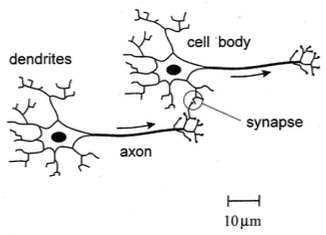
\includegraphics[width = 0.6 \linewidth]{images/biological neuron.png}
    \centering
    \caption{Composizione di due neuroni biologici.}
    \label{biological neuron}
\end{figure}
Da come possiamo notare, esistono vari componenti che costituiscono un 
neurone. In particolare, abbiamo i \emph{dendriti} che rappresentano gli ingressi di un 
neurone mentre le uscite sono rappresentare dagli \emph{assoni}. Su ogni assone viaggia 
un impulso elettrico generato dal neurone stesso quando questo si trova in uno 
stato attivo. Ogni neurone è connesso a migliaia di suoi simili ed ogni 
comunicazione fra questi avviene mediante le sinapsi. Quando l’impulso raggiunge 
proprio le sinapsi, questo provoca il rilascio di sostanze chimiche che attraversano 
la giunzioni ed entrano all’interno di altri neuroni. Ci sono due tipologie di sinapsi, 
eccitatori e inibitori. La prima tipologia permette di aumentare la probabilità che 
un neurone si attivi. Tale probabilità è determinata dal peso associato ad ogni 
sinapsi. Avendo multipli collegamenti, ogni neurone effettua una specie di somma 
pesata degli ingressi che, se maggiore di una determinata soglia, può provocare la 
sua attivazione. 

\section{Reti Neurali Artificiali}\label{Reti neurali}
Una rete neurale artificiale è un modello computazionale che, a partire da dei dati 
di input, riesce a produrre un output mediante un meccanismo ispirato a quello 
del cervello umano. Alla base di questa similitudine, tali reti prendono il nome di 
\emph{Artificial Neural Networks (ANN)}. Le prime reti neurali, nate attorno gli anni 
’50, basavano il loro funzionamento sui cosiddetti \emph{percettroni}, neuroni artificiali in 
grado di apprendere e di accumulare esperienza. Ogni rete neurale è composta da 
strati di neuroni, comunemente chiamati \emph{layers}. I dati di input saranno processati 
dai neuroni presenti nell’input layer e da qui, i risultati ottenuti, si propagheranno 
verso i layer nascosti (hidden layers) fino a raggiungere il layer finale di output (Fig. \ref{network structure}).
\begin{figure}[H]
    \centering
    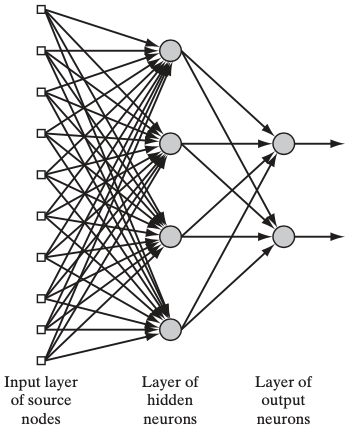
\includegraphics[width = 0.6 \linewidth]{images/netwrok structure.png}
    \centering
    \caption{Struttura di una rete neurale a più livelli.}
    \label{network structure}
\end{figure}
Una componente importante, riguarda la presenza di un insieme di valori 
$w=(w_{j1}, \dots, w_{jm})$ chiamati pesi. Ogni peso è rappresentato da un numero reale 
che riflette il grado di importanza di una data connessione, tra due neuroni, in 
una rete neurale. I pesi possono subire dei cambiamenti in base alla tipologia 
di apprendimento della rete. Una buona configurazione dei pesi riduce l’errore di 
predizione e pertanto migliora l’output del modello. Riprendendo il discorso 
dei neuroni, McCulloch e Pitts  \cite{Chakraverty2019} definirono un modello matematico in grado di 
rappresentarli. In particolare, il compito di ogni singolo neurone è rappresentato 
nella figura (\ref{neural neuron}).
\begin{figure}[H]
    \centering
    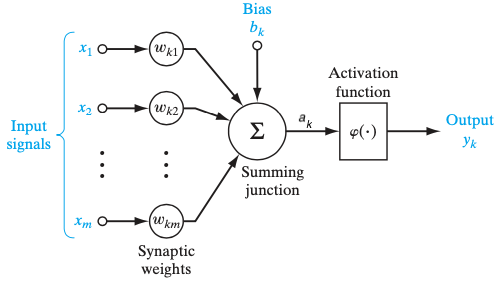
\includegraphics[width = \linewidth]{artificial neuron.png}
    \centering
    \caption{Neurone artificiale.}
    \label{neural neuron}
\end{figure}
Da come possiamo notare, un neurone è una semplice funzione non lineare 
che riceve in input una serie di input $X_{ji}$ e produce in output una variabile $y_k$. 
Il calcolo dell’output, di ogni singolo neurone, è composto da una sommatoria 
degli input, di segno positivo o negativo, moltiplicati prima con i corrispettivi 
pesi e successivamente sommati con una variabile, chiamata bias (pregiudizio), 
che corrisponde alla soglia di attivazione del neurone.
\begin{equation}\label{artificial}
    a_j = \sum_{i=0}^m w_{i}x_i + b_i 
\end{equation}
Una soglia è utile per determinare se l’informazione in ingresso “$x$” debba essere 
elaborata oppure scartata. Di solito vi è sempre un input $X_0=1$ che renderebbe 
il bias $ b_i $ uguale uguale al primo peso $W_0$, pertanto la formula (\ref{artificial}) può anche 
essere scritta come:
\begin{equation}\label{artificial without bias}
    a_j = \sum_{i=0}^m w_{i}x_i
\end{equation}
Per poter determinare il valore $y$, dopo aver ottenuto “$a$”, si utilizza una “\emph{funzione 
di attivazione}” non lineare $\varphi(\cdot)$:
\begin{equation}\label{activation function 1}
    y_j = \varphi(a) = \varphi\left(\sum_{i=0}^m w_ix_i\right)
\end{equation}
L’uscita $y$ determinerà l’attivazione del prossimo neurone. Se il valore ricevuto è 
maggiore di zero, allora il neurone si attiverà, altrimenti resterà spento.
\begin{equation}\label{activation function 2}
    y_j = \left\{
        \begin{array}{rl}
        1 & \mbox{if } a_j \geq 0 \\
        0 & \mbox{if } a_j < 0
        \end{array}
        \right.
\end{equation}
Esistono varie funzioni di attivazione, diverse sono elencate in figura (\ref{activation functions}).
\begin{figure}[H]
    \centering
    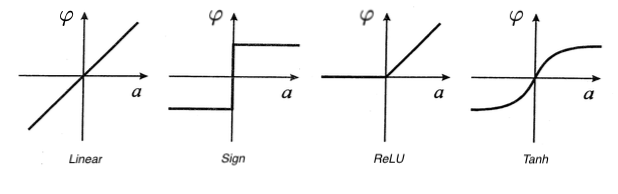
\includegraphics[width = \linewidth]{activation functions.png}
    \centering
    \caption{Varie funzioni di attivazione.}
    \label{activation functions}
\end{figure}
Grazie a questa massiccia interconnessione, le reti neurali artificiali sono in 
grado non solo di imitare il comportamento del cervello umano ma anche di 
svolgere diversi compiti grazie a una opportuna fase di apprendimento. 

\section{Algoritmi di apprendimento}
Lo scambio di dati tra i vari neuroni consente alla rete neurale di poter generalizzare 
anche con dati mai visti nel training set. Questo processo prende il nome di 
“\emph{Apprendimento}”. L’apprendimento di un modello di rete è tipicamente effettuato 
a partire da un insieme di dati di addestramento chiamato training test. All’interno 
di questi insiemi abbiamo la presenza di esempi formati da coppie $(x^j, y^j)$, con 
$j=1,…,n$, dove $y^j$ sta a rappresentare il valore di output desiderato in funzione 
del dato di input $x^j$. Per ricavare il valore target è necessario ricercare gli 
opportuni valori dei pesi, indispensabili a minimizzare l’errore commesso. La 
quantità dell’errore commesso, dal singolo neurone $j$, è esprimibile mediante (\ref{error function}):
\begin{equation}\label{error function 1}
    \emph{$e_j$}=(\hat{y}_j-y_j)^2
\end{equation}
Si può osservare che il calcolo di (\ref{error function 1}) è riconducibile alla somma dei quadrati 
residua tra il valore stimato $\hat{y}_j$ e quello desiderato $y_j$. L’errore totale derivato da 
tutta la rete è calcolabile prendendo in considerazione la \emph{Funzione di Errore}, a 
volte chiamata anche di \emph{Costo}, esprimibile dal calcolo della seguente formula:
\begin{equation}\label{error function}
    \emph{$E$}=\frac{1}{2}\sum_{j=1}^me_j
\end{equation}
dove $m$ rappresenta il numero totale di neuroni presenti nell’output layer.
La funzione di errore $E$ risulta essere molto importate nella fase di apprendimento in quanto misura la distanza 
dalla soluzione ottimale. In generale, la funzione di errore ha diversi minimi (Fig. \ref{minimum and maximum})
\begin{figure}[H]
    \centering
    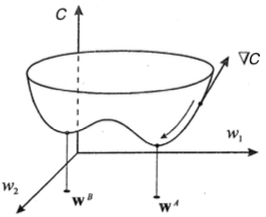
\includegraphics[width = 0.7\linewidth]{cost-function.png}
    \centering
    \caption{Esempio di minimo globale ($w^A$) e locale ($w^B$).}
    \label{minimum and maximum}
\end{figure}
Per ottenere un valore della funzione relativamente basso, l’obiettivo è racchiuso 
nella ricerca del minimo globale. Tale ricerca avviene in maniera iterativa, partendo 
da dei pesi a valori casuali, fino a definirne dei valori fissi. La ricerca dei pesi 
ottimali avviene mediante calcolo delle derivate parziali sulla funzione di errore, 
ovvero del suo vettore gradiente $\nabla{E}$ (\ref{gradient vector}). 
\begin{equation}\label{gradient vector}
    \nabla{E}[\vec{w}]\equiv\left[\frac{\partial E}{\partial w_{0}}, \frac{\partial E}{\partial w_{1}}, \dots, \frac{\partial E}{\partial w_{j}}\right]
\end{equation}
Questo vettore è utile a definire la direzione ed il verso della funzione di errore, 
in base al set di pesi considerato. Il calcolo delle derivate viene svolto da una ben 
nota tecnica presente allo stato dell'arte, chiamata \emph{Back Propagation} (discussa 
nella sezione \ref{BP} di questo elaborato). Una rete neurale artificiale può avere vari 
tipi di apprendimento: \emph{Supervisionato, Semi-Supervisionato, Non-Supervisionato} 
e con \emph{Rinforzo}. La scelta di quale usare dipende dalla tipologia della rete e dal 
suo campo di applicazione.

\subsection{Apprendimento Supervisionato}
In questa tipologia di apprendimento, l’input fornito alla rete contiene una serie di 
dati etichettati. L’apprendimento supervisionato è solitamente utilizzato sia nel 
conteso della classificazione, dove  si vuole mappare le etichette di input a quelle 
di output, che nel contesto della regressione, dove si mira a mappare l’input a un 
output continuo. La corretta associazione comporta una buona generalizzazione 
da parte del modello. L’apprendimento migliora grazie ad una continua variazione 
dei pesi. Questo tipo di apprendimento è svolto utilizzando la tecnica della 
\emph{Back-Propagation}. La complessità di questo tipo di apprendimento deriva dalla 
quantità di dati presenti nel training set. Affinché la rete riesca a generalizzare al 
meglio, il training set dev’essere composto da un numero di esempi adeguato. La 
giusta quantità di esempi è utile a prevenire spiacevoli situazioni di underfitting o 
di overfitting della rete.

\subsection{Apprendimento Non-Supervisionato}
Quando una rete neurale è sottoposta ad un simile apprendimento, questa riceve 
in input dei dati privi di etichettatura o non strutturati. Lo scopo della rete, 
o del modello, è quello di estrarne una rappresentazione e creare dei cluster 
rappresentativi. Ci sono delle tecniche a supporto di questa tipologia di apprendimento, 
una fra queste è la riduzione della dimensionalità che è applicata in fase 
di pre-elaborazione delle features avente l’obiettivo di eliminare il rumore dai dati 
quando questi sono presenti in grandi quantità. 

\subsection{Apprendimento Semi-Supervisionato}
Un set di input composto da dati etichettati e non, costituisce un sistema di apprendimento 
semi-supervisionato. Questa tipologia di apprendimento rappresenta 
un sistema che si interpone tra i due precedentemente spiegati. I modelli che fanno 
uso di questo approccio di solito utilizzano una piccola quantità di dati etichettati 
e una grande quantità di dati non etichettati. Tale apprendimento porta alla 
creazione di un modello più flessibile rispetto a quello ottenuto dall’apprendimento 
supervisionato.

\subsection{Apprendimento con Rinforzo}
L’ultimo tipo di apprendimento automatico è chiamato Apprendimento con 
Rinforzo. Il suo scopo è quello di costruire un sistema, comunemente chiamato 
\emph{agente}, che abbia l’obiettivo di migliorare le sue performance interagendo con 
l’ambiente che lo circonda. Il miglioramento dell’intero sistema avviene mediante 
dei feedback chiamati appunto rinforzi. Quest’ultimi non hanno nulla a che fare 
con etichette o valori di verità, ma rappresentano un livello di qualità delle azioni 
intraprese dal sistema. Pertanto, differentemente da un sistema supervisionato, 
non ci sono mappature tra l’input e l’output.

\subsection{Algoritmo di Back-Propagation}\label{BP}
Il termine \emph{Back-Propagation} è stato introdotto una prima volta quando si è 
trattato l’argomento dell’apprendimento Supervisionato. Una prima definizione 
del termine venne data nel 1986 in \cite{03}. L’algoritmo di Back-Propagation agisce 
durante la fase di training del modello, che a sua volta si suddivide in due fasi:
\begin{enumerate}
    \item \emph{Fase in avanti (forward)}: i dati si propagavano dai neuroni di input fino 
    a raggiungere i neuroni di output. I pesi sono fissati e i cambiamenti sono 
    limitati.
    \begin{figure}[H]
        \centering
        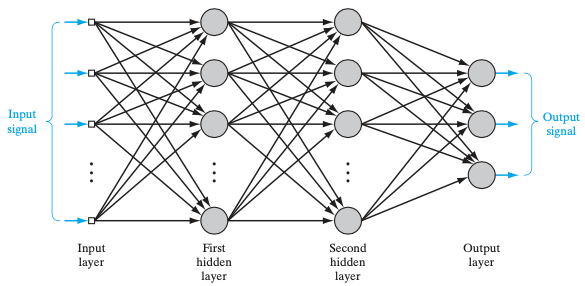
\includegraphics[width = \linewidth]{feedforward.png}
        \centering
        \caption{Esempio fase di propagazone dei dati in avanti di una rete \emph{feedforward}.}
        \label{feedforward net}
    \end{figure}
    \item \emph{Fase in indietro (backward)}:  si confronta il risultato ottenuto, da un primo 
    step in avanti, con il risultato atteso. Tale valore rappresenterà l’errore 
    commesso, descritto in precedenza dalla funzione di errore $E$ (\ref{error function}). A questo 
    punto, tale errore si propagherà indietro nella rete. Questo meccanismo è 
    utile ad adeguare i vari pesi presenti nella rete affinché le prossime iterazioni 
    diano un errore relativamente basso (caso ottimale in cui l’output stimato è 
    simile all’output desiderato).
    \begin{figure}[H]
        \centering
        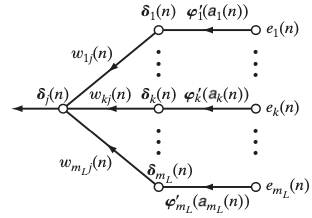
\includegraphics[width = 0.7\linewidth]{BP.png}
        \centering
        \caption{Esempio fase di retropropagazione degli errori.}
        \label{BP error}
    \end{figure}
\end{enumerate}
Sappiamo che una minima variazione ai pesi e al bias comporta allo stesso modo 
una variazione della funzione di errore E. Tralasciando un’attimo il bias, il discorso 
che segue è incentrato sulla gestione dei pesi. L’algoritmo di Back-propagation 
applica una correzione chiamata {\bfseries{Delta Rule ($\Delta{W_{ji}}$)}}  ad ogni peso $w_{ji}$, andando 
a calcolare, tramite la regola della \emph{Chain Rule} \ref{chain rule}, la derivata parziale della funzione 
di errore $E$, rispetto alla derivata della parziale del peso $w_{ji}$ in considerazione.
\begin{equation}\label{chain rule}
    \frac{\partial E}{\partial w_{ji}} = \frac{\partial E}{\partial e_{j}} 
    \frac{\partial e_{j}}{\partial y_{j}}
    \frac{\partial y_{j}}{\partial a_{j}}
    \frac{\partial a_{j}}{\partial w_{ji}}
\end{equation}
dove:
\begin{equation}\label{derivation solved 1}
    \frac{\partial E}{\partial e_{j}} = e_j
\end{equation}
\begin{equation}\label{derivation solved 2}
    \frac{\partial e_{j}}{\partial y_{j}} = -1
\end{equation}
\begin{equation}\label{derivation solved 3}
    \frac{\partial y_{j}}{\partial a_{j}} = \varphi_j^{'}(a_j)
\end{equation}
\begin{equation}\label{derivation solved 4}
    \frac{\partial a_{j}}{\partial w_{ji}} = y_i
\end{equation}
Ogni elemento definito dalla chain rule sarà utile, oltre che a formare il vettore 
del gradiente $\nabla{E}$ (\ref{gradient vector}), a determinare la direzione di ricerca all’interno dello spazio 
dei pesi, per un singolo peso $w_{ji}$. Questa operazione, in letteratura, è nominata 
come \emph{“Discesa del gradiente”}. Ricapitolando, la (\ref{chain rule}) diventa:
\begin{equation}\label{chain rule update}
    \frac{\partial E}{\partial w_{ji}} = -e_j\varphi_j^{'}(a_j)y_i
\end{equation}
Giunti a questo punto, è possibile calcolare la \emph{Delta Rule} ($\Delta{W_{ji}}$) sul peso $w_{ji}$:
\begin{equation}\label{delta rule 1}
    \Delta{W_{ji}} = -\alpha \frac{\partial E}{\partial w_{ji}}
\end{equation}
dove $-\alpha$ simboleggia un parametro, chiamata \emph{Learning Rate}, che rappresenta 
un indicatore di velocità di apprendimento della rete. Il segno negativo è utile 
per agevolare la discesa del gradiente affinché si riduca il valore della funzione di
errore $E$. Dalla (\ref{delta rule 1}) possiamo definire il \emph{gradiente locale $\delta_j$}:
\begin{eqnarray}\label{local gradient of output layer}
    \delta_j & = & \frac{\partial E}{\partial a_{j}} \nonumber \\
             & = & \frac{\partial E}{\partial e_{j}} \frac{\partial e_{j}}{\partial y_{j}} \frac{\partial y_{j}}{\partial a_{j}} \nonumber \\
             & = & e_j\varphi_j^{'}(a_j)
\end{eqnarray}
Il gradiente locale sta ad indicare i cambiamenti richiesti nei pesi e questo dipende 
dalla tipologia di neurone:
\begin{enumerate}
    \item Se il neurone \emph{j} è un neurone di output, $\delta_j$ è uguale al prodotto della derivata 
    $\varphi_j^{'}(a_j)$ e il singolo errore $e_{j}$, entrambi associati al neurone $j$ (\ref{local gradient of output layer});
    \item Se il neurone \emph{j} è un neurone nascosto, $\delta_j$ è uguale al prodotto tra la derivata 
    $\varphi_j^{'}(a_j)$ e la sommatoria dei vari $\delta$ calcolati sui neuroni posti nel layer nascosto, 
    o nel layer di output, connessi al neurone \emph{j} (\ref{local gradient of hidden neuron}).
    \begin{equation}\label{local gradient of hidden neuron}
        \delta_j = \varphi_j^{'}(a_j)\sum_{k}\delta_kw_{kj}
    \end{equation}
\end{enumerate}
Sostituendo in (\ref{chain rule update}) la (\ref{local gradient of output layer}), possiamo modificare la (\ref{delta rule 1}) in:
\begin{equation}\label{delta rule 2}
    \Delta{W_{ji}} = -\alpha \delta_jy_i 
\end{equation}
Infine, grazie alla definizione della \emph{Delta Rule}, nell’iterazione $n+1$ sarà possibile 
aggiornare il peso $w_{ji}$ in questione, rispetto all’iterazione $n$ precedente:
\begin{equation}\label{weight change}
    w_{ji}(n+1) = w_{ji}(n)+\Delta{w_{ji}(n)}
\end{equation}
In precedenza, si era preferito mettere da parte il concetto di bias per concentrarci 
maggiormente sui pesi. Essendo la funzione di errore sensibile anche al cambiamento 
del bias, l’algoritmo di back-propagation ha lo scopo di aggiornare anche i 
vari bias esistenti integrando, nel vettore gradiente $\nabla{E}$, le derivate parziali della 
funzione di Errore rispetto al bias $b$:
\begin{equation}\label{gradient vector with bias}
    \nabla{E}[\vec{b}]\equiv\left[\frac{\partial E}{\partial b_{0}}, \frac{\partial E}{\partial b_{1}}, \dots, \frac{\partial E}{\partial b_{j}}\right]
\end{equation}
I successivi calcoli sono identici a quelli dell’aggiornamento dei pesi. Il processo 
di back-propagation avviene in maniera iterativa e si ferma quando vengono 
soddisfatte le seguenti caratteristiche:
\begin{enumerate}
    \item Raggiungimento del numero massimo di epoche;
    \item L’errore è più basso della soglia;
    \item Non vi è nessun cambiamento dei pesi.
\end{enumerate}

\section{Tipologie di reti neurali}
Esistono diverse tipologie di reti neurali, tra queste abbiamo:
\begin{itemize}
    \item \emph{Reti neurali feed forward (FNN)}
    \item \emph{Reti neurali ricorrenti (RNN)}
    \item \emph{Reti profonde (DNN)}
    \item \emph{Reti convoluzionali (CNN)}
\end{itemize}
Nel seguente elaborato verranno trattate solamente le reti neurali convoluzionali 
ma, prima di introdurle, al fine di capire il loro funzionamento, è necessario 
introdurre prima le reti neurali feed-forward, dette anche reti neurali a catena 
aperta.

\subsection{Reti neurali Feed-Forward}
Per facilitare la comprensione del funzionamento di una comune rete neurale, 
si potrebbe partire dallo studio del comportamento di una feed-forward neural 
network. Questa tipologia di rete può essere vista come una funzione matematica 
non lineare capace di trasformare dei dati di input $x=(x_1, \dots, x_m)$, in dati in 
output $y=(y_{j1}, \dots, y_{jn})$. Quello che accade è quindi una transizione delle variabili 
indipendenti ($X_j$) in variabili dipendenti($Y_j$). Possiamo quindi considerare la 
rete come una funzione nella forma $y = y(x;w)$, dove $y$ sta a rappresentare una funzione di $x$ 
e che a sua volta è parametrizzata da $w$. In una rete feed-forward, il 
processo di calcolo è unilaterale, ovvero procede solamente in avanti, raggiungendo 
l’ultimo layer. Rispetto a una rete semplice, una rete feedforward può essere 
composta da più layer nascosti in cui vi sono più neuroni nascosti. L’aggiunta 
di un numero sostanziale di layer nascosti può aiutare ad estrarre statistiche di 
ordine superiore dai dati di input. Secondo \cite{04}, la presenza di più connessioni 
sinaptiche tra i neuroni, provoca una maggiore iterazione tra questi che a sua 
volta aiuta alla rete a raggiungere una prospettiva globale. Una rete che ha più di 
un layer nascosto, e quindi probabilmente con un alto numero di connessioni, in 
gergo è chiamata rete \emph{fully connected}. Al contrario, se alcuni collegamenti sono 
assenti, tale tipologia di rete viene chiamata \emph{partially connected}.

\subsection{Reti neurali Convoluzionali}\label{RNC}
Una rete neurale convoluzionale (CNN o ConvNet) è una tipologia di rete feed-
forward che si sta affermando come stato dell’arte per una svariata gamma di 
applicazioni nel campo della computer vision. Una loro prima diffusione avvenne 
negli anni ’90 grazie a uno studio di LeCun e Boser \cite{NIPS1989_53c3bce6}. L’architettura delle CNN 
si distinguono grazie al numero di layer presenti.  La loro particolarità sta nel 
rilevare i tratti più rilevanti e di apprendere i pattern, il tutto con un alto grado di 
invariata rispetto a traslazione, ridimensionamento, inclinazione e altre forme di 
distorsione. I primi strati hanno il compito di estrarre le features di basso livello, 
come per esempio i bordi o i blob, al contrario, gli ultimi strati hanno lo scopo di 
estrarre le features di alto livello tipo i contorni, classificazione, riconoscimento 
etc. All’interno di una rete convoluzionale possiamo riconoscere due tipologie di 
neuroni:
\begin{itemize}
    \item \emph{Neuroni di elaborazione}: hanno lo scopo di elaborare una sezione specifica 
    dell’immagine, comunemente chiamata campo ricettivo, utilizzando 
    un’operazione di \emph{convoluzione};
    \item \emph{Neuroni di aggregazione}: hanno lo scopo di eseguire un'operazione di \emph{pooling}.
\end{itemize}
I neuroni contenuti in uno strato adibito alla convoluzione, e quelli completamente 
connessi, dispongono di funzioni di attivazione e di pesi, quest’ultimi sottoposti a 
processo di aggiornamento durante la fase di apprendimento. Per quanto riguarda 
gli strati di pooling, questi non dispongo di alcun tipi di peso. Riassumendo, 
le operazioni svolte dalle CNN sono essenzialmente quattro: {\bfseries{Convoluzione}}, {\bfseries{Non 
Linearità (ReLU)}}, {\bfseries{Pooling (o Sub Sampling)}} e {\bfseries{Classificazione}} (nei layer 
fully connected). 
\begin{figure}[H]
    \centering
    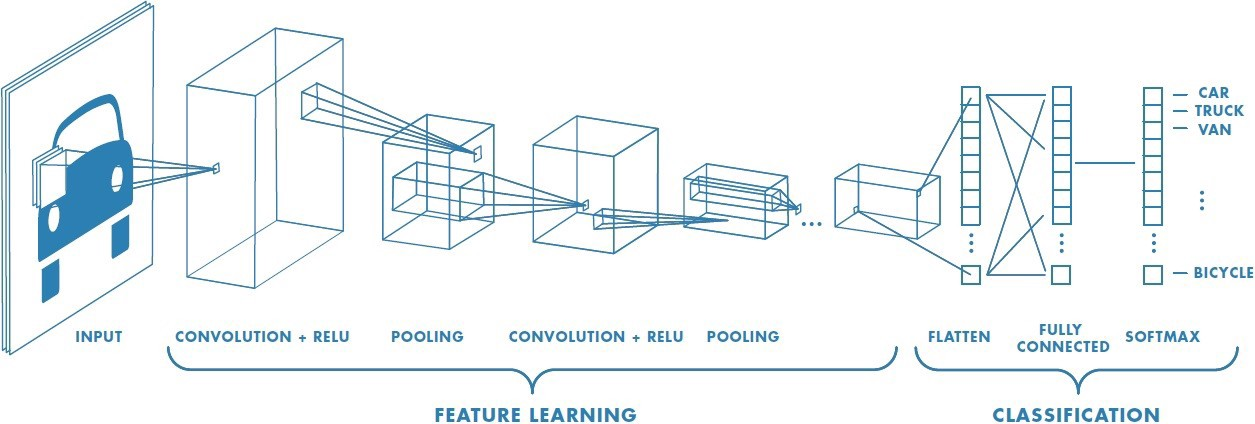
\includegraphics[width = \linewidth]{cnn complete.png}
    \centering
    \caption{Esempio di architettura di una rete CNN.}
    \label{CNN complete}
\end{figure}

\subsubsection{Convoluzione}
Lo scopo del layer di convoluzione è quello di attuare un’operazione di {\bfseries{feature 
extraction}}. In questa fase ogni neurone prende in input un campo ricettivo 
locale del layer precedente e da qui ne estrae le feature locali. Un filtro, che in 
gergo prende il nome di {\bfseries{\emph{kernel}}}, trasla sull’immagine originale con l’intenzione di 
creare una feature map mediante moltiplicazione tra i valori presenti nel filtro, 
corrispondenti ai pesi, e la regione dell’immagine in cui si trova. Di seguito, i 
valori di ogni feature map sono calcolati tramite la seguente formula:
\begin{equation}\label{sum convolution}
    G[m,n] = (f*h)[m,n] = \sum_j\sum_kh[j,k]f[m-j,n-k]
\end{equation}
dove:
\begin{itemize}
    \item $f$: immagine in input;
    \item $h$: kernel;
    \item $m,n$: indici di riga e colonna del campo ricettivo dell'immagine;
    \item $i,j$: indici di riga e colonna del kernel;
\end{itemize}
\begin{figure}[H]
    \centering
    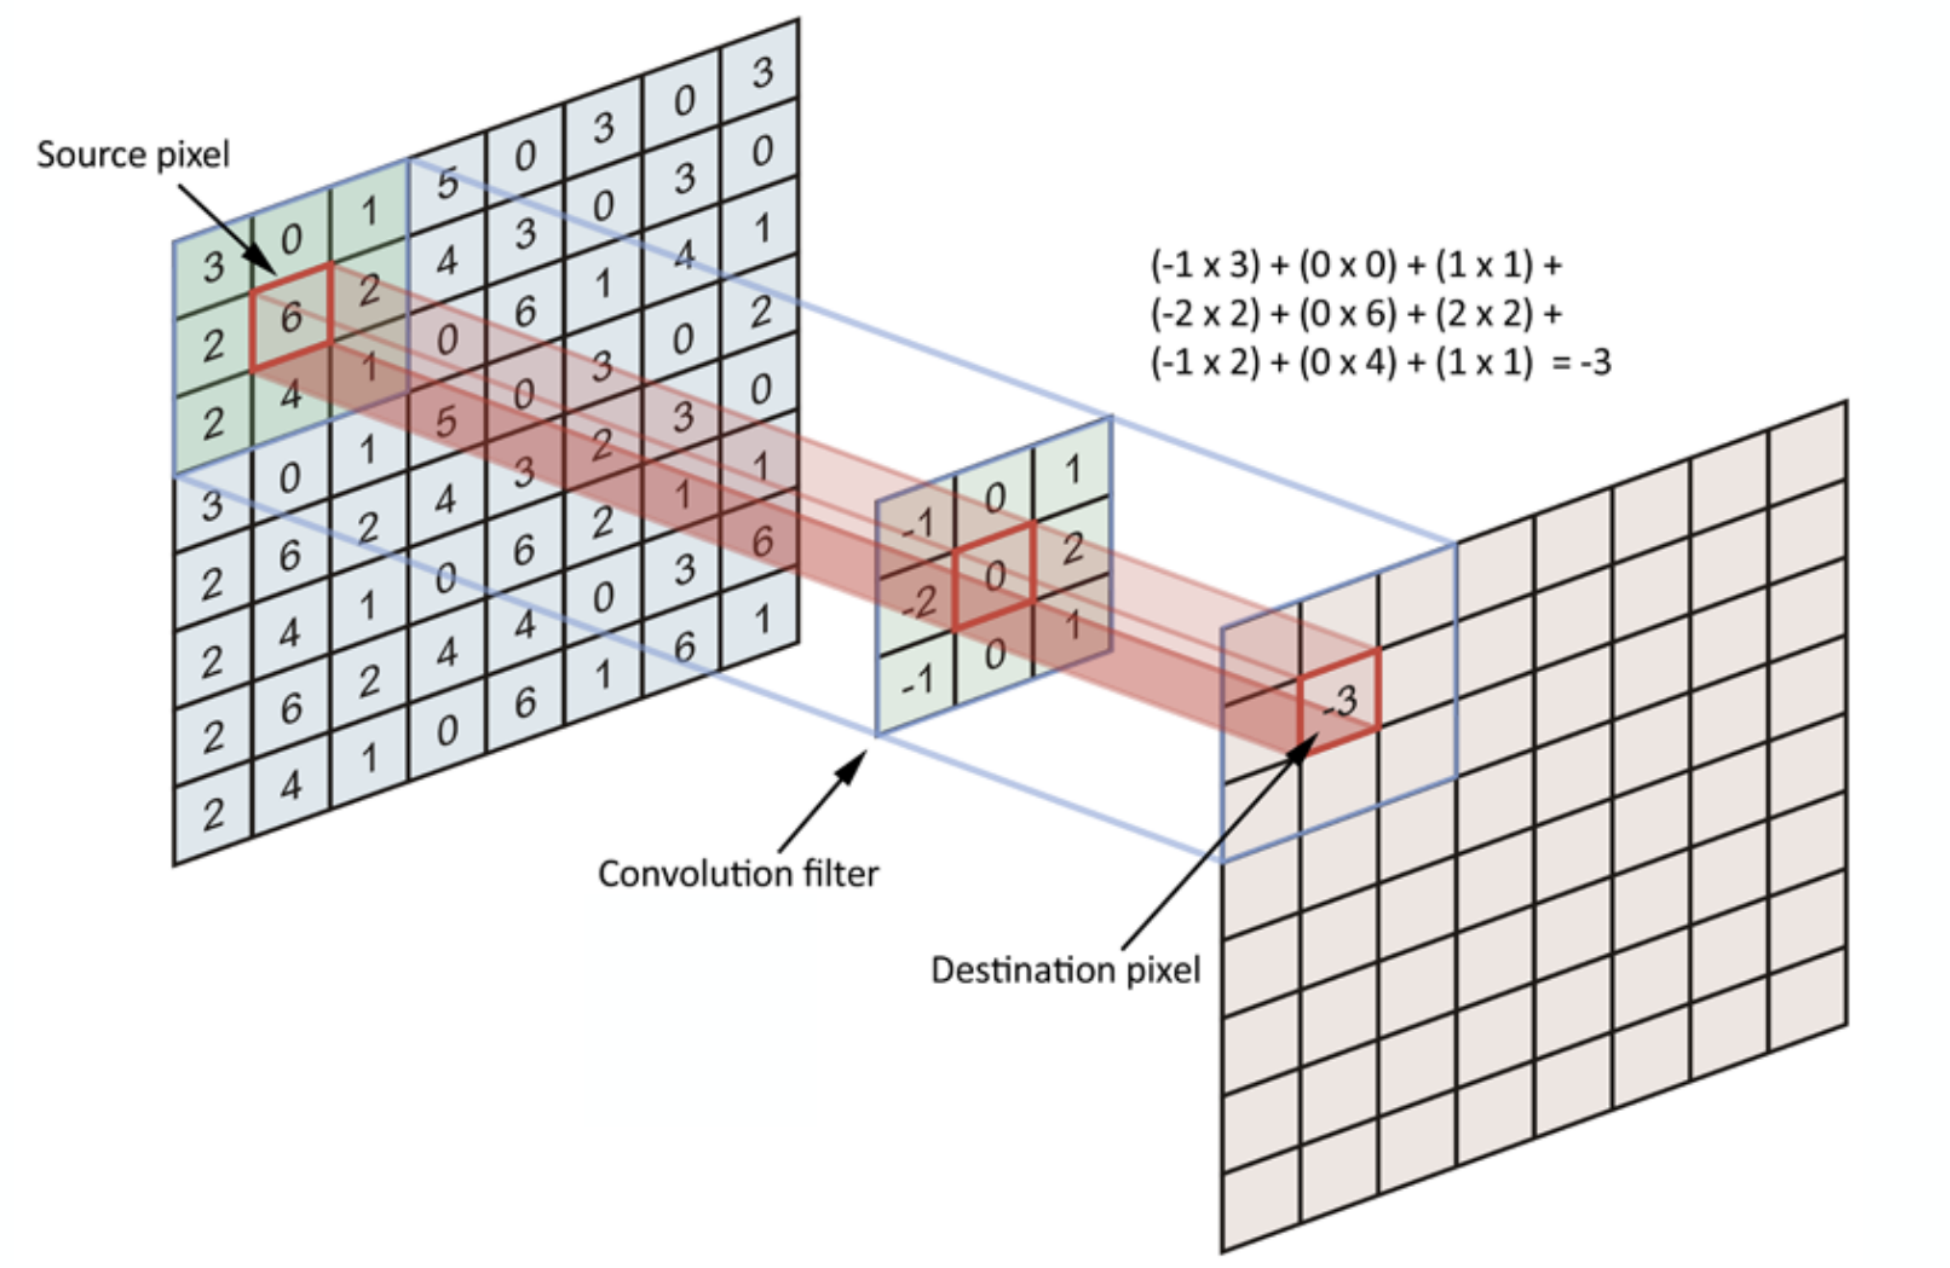
\includegraphics[width = 0.8\linewidth]{convolution.png}
    \centering
    \caption{Esempio di dimensione filter e di campo ricettivo.}
    \label{filter dimension}
\end{figure}
Dopo aver posizionato il filtro su un campo ricettivo, vero preso ogni valore dal 
kernel e moltiplicato con i valori corrispondenti al campo ricettivo dell’immagine. 
Successivamente, il valore risultante verrà inserito nella giusta posizione della 
feature map. Il numero di feature map sarà uguale al numero di filtri applicato 
sull’immagine. La generazione di ogni feature map dipende da quattro tipi di 
parametri, detti 
\emph{iperparametri}:
\begin{enumerate}
    \item \emph{Dimensione dei filtri}: pari alla dimensione del campo ricettivo ovvero della 
    porzione dell’immagine che si vuole analizzare;
    \item \emph{Profondità (depth)}: numero di filtri “$N$” usati durante la convoluzione 
    ($H \times W \times N$). Ogni filtro produrrà una propria feature map;
    \begin{figure}[H]
        \centering
        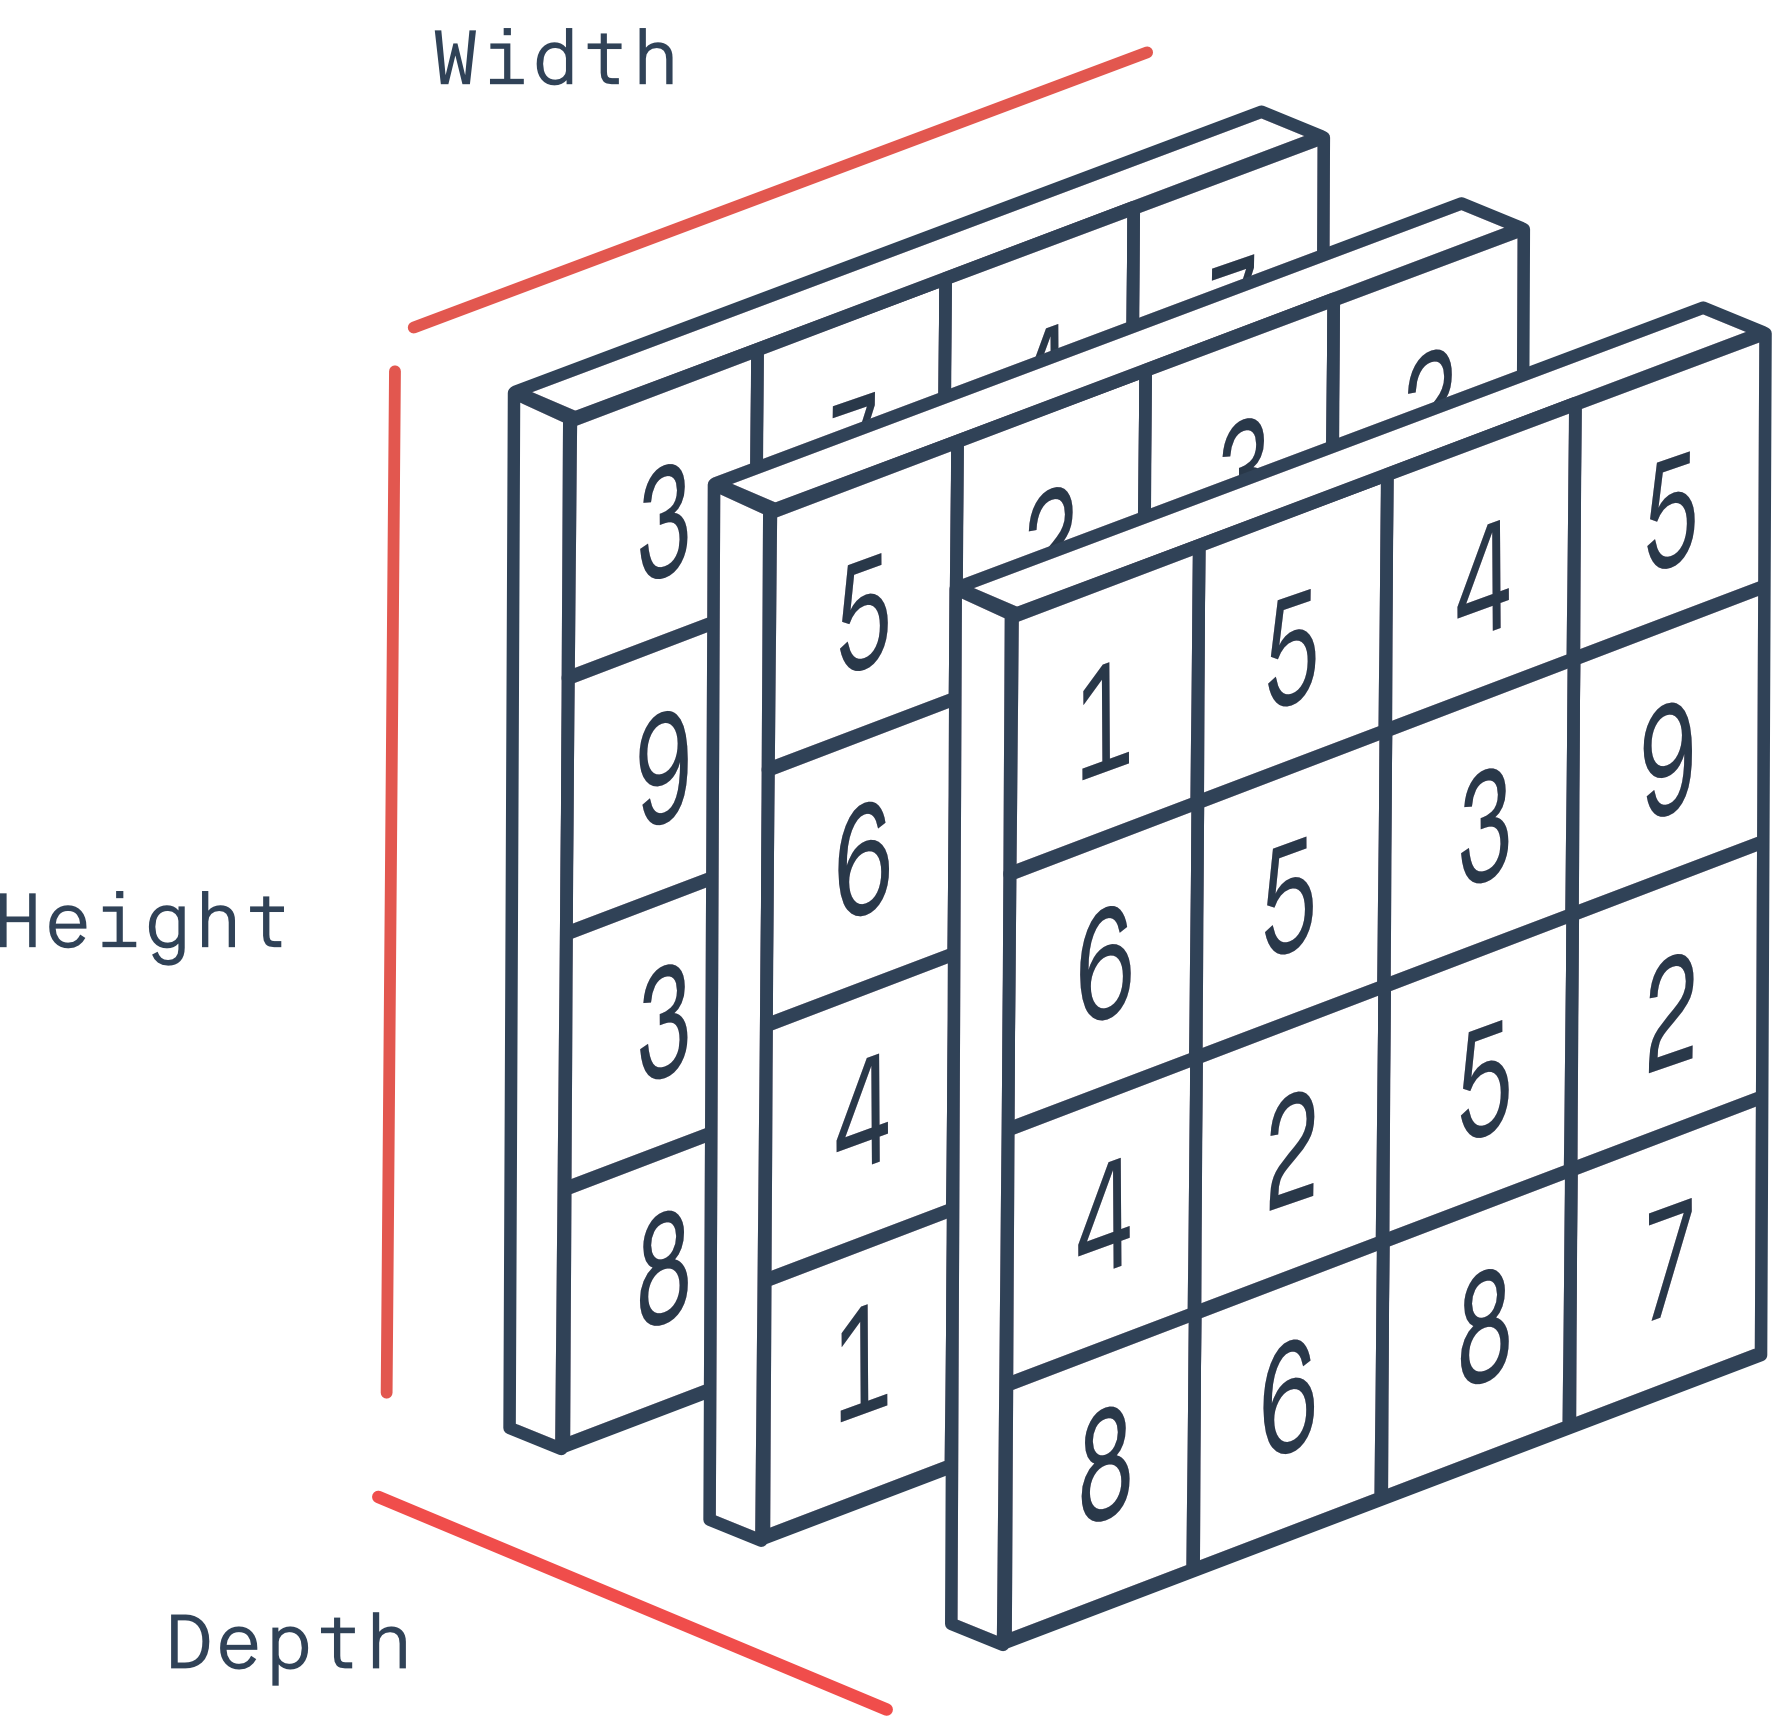
\includegraphics[width = 0.5\linewidth]{filter.png}
        \centering
        \caption{Esempio di profondità composto da più filtri.}
        \label{filters depth}
    \end{figure}
    \item \emph{Passo (stride)}: rappresenta il numero di pixel su cui viene fatto traslare il 
    kernel ogni volta che esegue una moltiplicazione. Per ottenere una buona 
    feature map è consigliato avere un valore di stride relativamente basso;
    \begin{figure}[H]
        \centering
        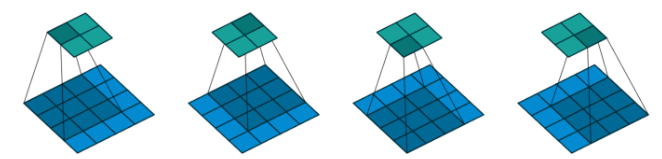
\includegraphics[width = \linewidth]{stride.png}
        \centering
        \caption{Esempio convoluzione con kernel=3x3 e stride=1.}
        \label{stride}
    \end{figure}
    \item \emph{Riempimento (Padding)}: affinché venga generata una corretta feature map 
    di dimensioni pari ($padding=1$) o maggiore ($padding>1$) a quella dell’immagine 
    di partenza, la matrice dell’immagine deve essere riempita di valori uguali, 
    esempio di zeri, presso le sue estremità.
    \begin{figure}[H]
        \centering
        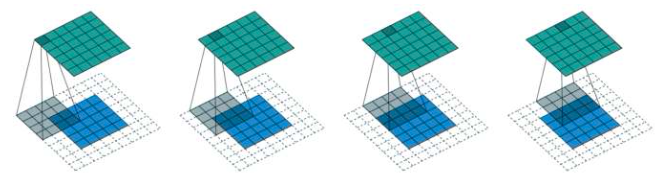
\includegraphics[width = \linewidth]{padding and stride.png}
        \centering
        \caption{Esempio convoluzione con kernel=4x, padding=2 e stride=1.}
        \label{padding e stride}
    \end{figure}
\end{enumerate}
La scelta degli iperparametri non è standard ma dipende maggiormente dalla 
tipologia dei dati a disposizione.

\subsubsection{Rectified Linear Unit (ReLU)}
Ogni feature map, dopo la convoluzione, è composta da dei valori positivi e negativi. 
Come brevemente accennato in (\ref{Reti neurali}), esistono varie funzioni di attivazione che, in 
base all’input ricevuto, decidono se attivare o disattivare un neurone. La 
funzione di attivazione maggiormente usata è la ReLU (Rectified Linear Unit). 
Questa funzione esegue delle operazioni non lineari ponendo a zero tutti i valori 
negativi e lasciando invariati i valori positivi, generando in questo modo delle 
attivazioni sparse.  L’operazione prende il nome di element-wise su tutti i pixel. 
L’implementazione di questa funzione, rispetto alle sue concorrenti, è utile ad accelerare 
il processo di apprendimento (backpropagation) del modello semplificando 
le operazioni nei vari layer.
\begin{figure}[H]
    \centering
    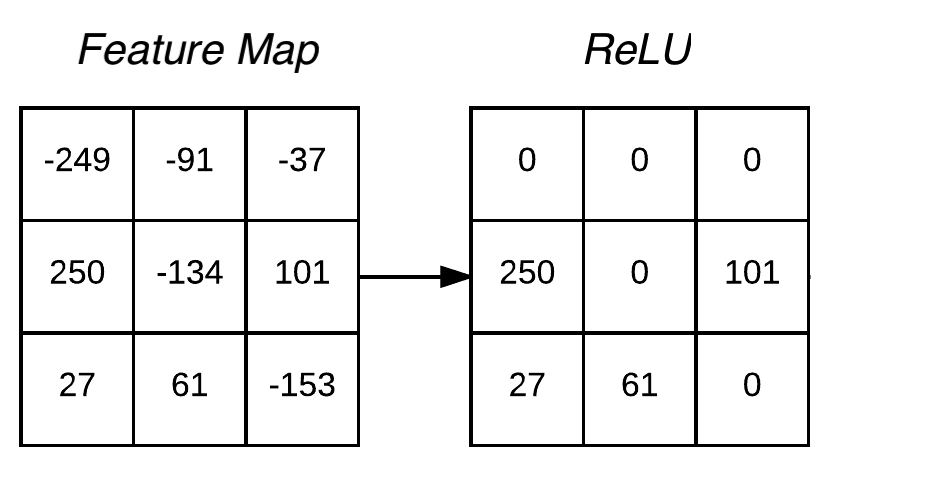
\includegraphics[width = 0.8\linewidth]{relu.png}
    \centering
    \caption{Esempio funzione di attivazione ReLU sui valori di una feature map.}
    \label{relu}
\end{figure}
Rispetto alla sigmoide, la funzione ReLU pone a zero la derivata di un numero 
negativo, mentre per i numeri positivi la derivata è uguale a uno evitando la 
saturazione del gradiente.

\subsubsection{Pooling}
La tecnica di Pooling, chiamata anche di subsampling o downsamping, ha il 
compito di ridurre la dimensionali di ogni feature map mantenendo però le 
informazioni più importanti. Il funzionamento di basa nel far scorrere una finestra, 
senza alcun tipo di valore o peso al suo interno, di dimensione inferiore rispetto 
alla grandezza della feature map, con lo scopo di aggregare i valori sottostanti. 
Esistono varie operazioni di aggregazione, le più comuni sono: somma, massimo, 
minimo e media. Così come la convoluzione, anche qui gli iperparametri Stride 
e Kernel size, entrambi solitamente uguale a 2, sono fondamentali al fine di gestire 
la finestra sovrastante. Ogni neurone, nello strato di pooling, è connesso a un 
numero limitato di neuroni nello strato precedente
\begin{figure}[H]
    \centering
    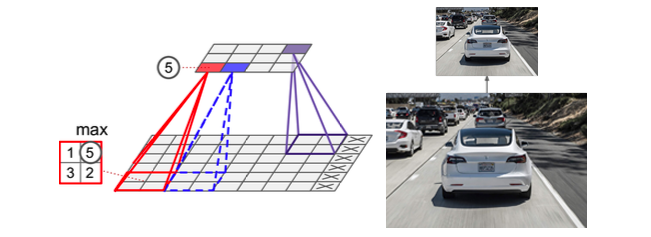
\includegraphics[width = \linewidth]{pooling tesla.png}
    \centering
    \caption{Esempio funzione di operazioni di pooling su una feature map.}
    \label{pooling}
\end{figure}
In (Fig. \ref{pooling}), applicando al funzione di \emph{Max-Pooling} al campo ricettivo in 
basso a sinistra, verrà selezionato il valore 5 che sarà propagato al prossimo 
layer. Avendo uno stride pari a 2, la matrice prodotta avrà una dimensione 
uguale alla metà della matrice di partenza (subsamplig),  che in questo caso è 
stata arrotondata per difetto. La riduzione delle dimensioni a sua volta riduce 
il numero di operazioni di calcolo, l’occupazione della memoria e il numero di 
parametri, limitando anche il rischio di overfitting in quanto si ha un numero 
minore di paramenti da apprendere. La funzione di Max-Pooling introduce quella che viene 
chiamata \emph{invarianza}, fattore importante che non permette ai cambiamenti di 
stravolgere il risultato finale, aggiungendo robustezza ai dati.

\subsubsection{Fully Connected}
Il layer \emph{Fully Connected (FC)} è una tradizionale \emph{Multilayer Perceptron (MLP)} 
che include una funzione di attivazione \emph{Softmax} nel layer di output. Lo scopo di 
tale layer è quello di utilizzare le feature estratte, dagli strati precedenti, in modo 
da predire le loro classi di appartenenza precedentemente fornite nel training 
set. Un vettore di numeri reali conterrà tutte le predizioni che, se sommate tra 
loro, produrranno un valore uguale a uno. Quest’ultimo passaggio sarà possibile 
grazie all’utilizzo di una funzione chiamata Softmax, posta alla fine dell’intera 
rete convoluzionale, che è in grado di “schiacciare” un vettore K-dimensionale 
a valori reali arbitrali, in un vettore K-dimensionale a valori reali, compresi nel 
range $(0,1)$. 

\section{Utilizzi delle reti neurali}
L’introduzione delle reti neurali, sia nel campo della computer vision che del deep 
learning, ha portato vari benefici nel risolvere problemi complessi nella vita reale. 
Il supporto offerto da questi sistemi è basato su tecniche di elaborazione delle 
immagini in grado di estrarre diverse informazioni utili per un determinato scopo. 
I task principali, eseguiti su un’immagine, possono essere:
\begin{itemize}
    \item \emph{Image classification}: viene effettuata un’analisi dell’immagine con lo scopo 
    di assegnare un’etichetta in base al suo contenuto;
    \item \emph{Object detection}: analisi degli elementi presenti all’interno di un’immagine;
    \item \emph{Image segmentation}: estrazione di regioni di interesse che identificano il 
    target in base al contesto;
    \item \emph{Face recognition}: basato sul riconoscimento facciale delle persone;
    \item \emph{Action recognition}: analisi incentrata sull’identificazione e sulla descrizione 
    di azioni compiute da parte di soggetti che interagiscono nel tempo e nello 
    spazio circostante;
    \item \emph{Visual Relationship Detection}: analisi mirata alla relazione che intercorre 
    tra gli oggetti presenti nell’immagine;
    \item \emph{Emotion Recognition}: processo atto a identificare le emozioni umane mediante 
    vari fattori come quello vocale e/o visivo;
    \item \emph{Image editing}: analisi delle immagini che portano l’algoritmo a riconoscere 
    le parti più rilevanti di un’immagine, come per esempio quelle più sensibili, 
    ed a attuare delle specifiche azioni, come ad esempio il loro oscuramento.
\end{itemize}
Il presente elaborato farà riferimento solamente alle prime tre tecniche, soffermandosi 
maggiormente sull’object detection e la semantic segmentation (branca 
dell’image segmentation).

\subsection{Object Detection}
L’object detection costituisce la base per risolvere compiti di visione complessi, 
o di alto livello, come la segmentazione, comprensione della scena, tracciamento 
degli oggetti, rilevamento degli eventi e riconoscimento delle attività. La tecnica 
di object detection supporta un ampio range di applicazioni, tra queste abbiamo 
la visione robotica, sicurezza, guida autonoma, segnali stradali, interazione uomo 
macchina, recupero delle immagini basato sui contenuti, videosorveglianza, realtà 
aumentata e ambito medico. Dal grafico \ref{obj det performance} possiamo vedere che dopo l’anno 
2012, periodo corrispondente all’introduzione del deep learning, le prestazioni 
della tecnica di object detection aumentarono notevolmente.
\begin{figure}[H]
    \centering
    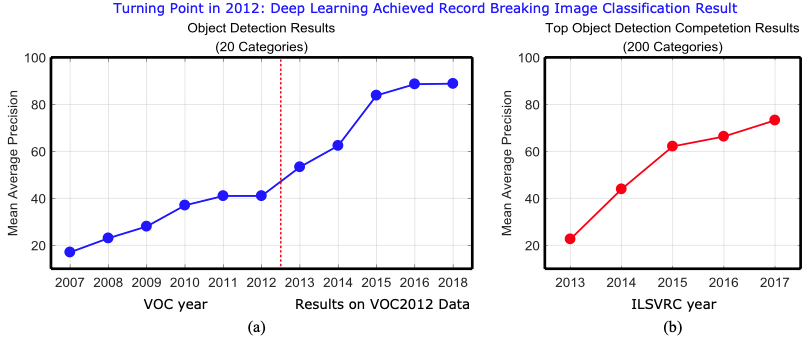
\includegraphics[width = \linewidth]{obj detection performance.png}
    \centering
    \caption{(a) Risultati object detection, in termini di mean average Precision, nelle competizioni VOC2007-2012 e (b) risultati della competizione per il rilevamento degli oggetti in ILSVRC2013-2017 su un numero di categorie maggiore}
    \label{obj det performance}
\end{figure}
Ogni oggetto è caratterizzato dalle sue proprietà come colore, forma, texture 
o altri tratti. Lo scopo della tecnica può essere visto come un problema di 
classificazione in grado di definire se un’immagine contiene un oggetto e, in caso 
affermativo, indicarne la posizione nell’immagine mediante l’utilizzo di un riquadro 
di delimitazione chiamato bounding box (Fig. \ref{object detection}). 
\begin{figure}[H]
    \centering
    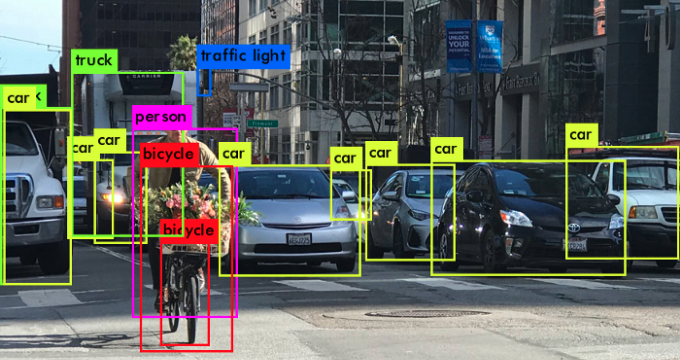
\includegraphics[width = 0.9\linewidth]{object detection.png}
    \centering
    \caption{Esempio di object detection.}
    \label{object detection}
\end{figure}
Se invece di un’immagine si sta elaborando un insieme di frame, come un video, 
allora lo scopo è quello di tracciare la posizione e  la dimensione dell’oggetto in 
tutti i frame (tecnica comunemente chiamata object tracking). Il rilevamento 
degli oggetti generici è strettamente correlato a:
\begin{enumerate}
    \item \emph{Segmentazione Semantica}: ha lo scopo di assegnare a ciascun pixel dell’immagine 
    un’etichetta corrispondente ad una classe (Fig. \ref{segmentation} (a));
    \item \emph{Instance segmentation}: tecnica che, al contrario della segmentazione semantica, 
    mira a distinguere diverse istanze appartenenti alla stessa classe di 
    oggetti (Fig. \ref{segmentation} (b)).
\end{enumerate}
\begin{figure}[H]
    \centering
    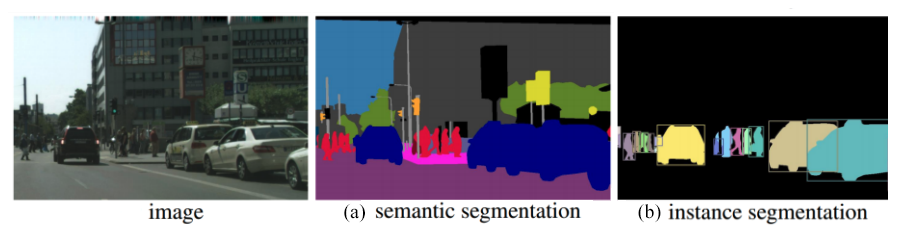
\includegraphics[width = \linewidth]{segmentation.png}
    \centering
    \caption{Problemi di riconoscimento relativi al rielvamento di automobili e pedoni: (a) Pixel-wise semantic segmentation, (b) Instance level semantic segmentation. }
    \label{segmentation}
\end{figure}
Uno dei principali obiettivi in questo campo è scegliere le feature che sono 
più caratteristiche dell’oggetto ricercato o, in altre parole, che sono altamente 
discriminanti, in modo da ottenere dei buoni risultati da parte del classificatore. Un 
aspetto fondamentale da tenere in considerazione è la complessità computazionale 
a cui i sistemi vanno incontro \cite{cyganek2013object}. I primi modelli di object detection basavano 
il loro funzionamento su delle feature estratte a mano \cite{viola2001rapid} \cite{dalal2005histograms}. Purtroppo, questi 
modelli erano molto lenti, imprecisi e non erano in grado di riconoscere i dati mai 
visti in precedenza. Le reti neurali convoluzionali (CNN) e del deep learning hanno 
cambiato il panorama della percezione visiva. Il problema di object detection è 
generalmente visto come un problema di apprendimento supervisionato. Nella 
computer vision sono stati raggiunti traguardi importanti negli ultimi dieci anni, 
tuttavia ci sono ancora grandi sfide da superare. Di seguito sono riportate alcune 
delle sfide chiave affrontate dalle reti neurali \cite{zaidi2021survey}:
\begin{itemize}
    \item \emph{Variabilità Intra-classe}: problematica che si verifica quando delle istanze appartenenti allo stesso oggetto differiscono pur appartenendo alla stessa classe. Nello specifico, questa problematica può essere suddivisa in due tipi \cite{liu2020deep}:
    \begin{enumerate}
        \item \emph{Fattori intrinseci}: multipli oggetti possono appartenere ad una stessa 
        categoria. A loro volta, queste istanze possono essere differenti in 
        termini di colore, consistenza, materiale, forma e dimensione, come per 
        esempio la categoria automobile (Fig. \ref{auto}):
        \begin{figure}[H]
            \centering
            \hspace*{1.5cm}
            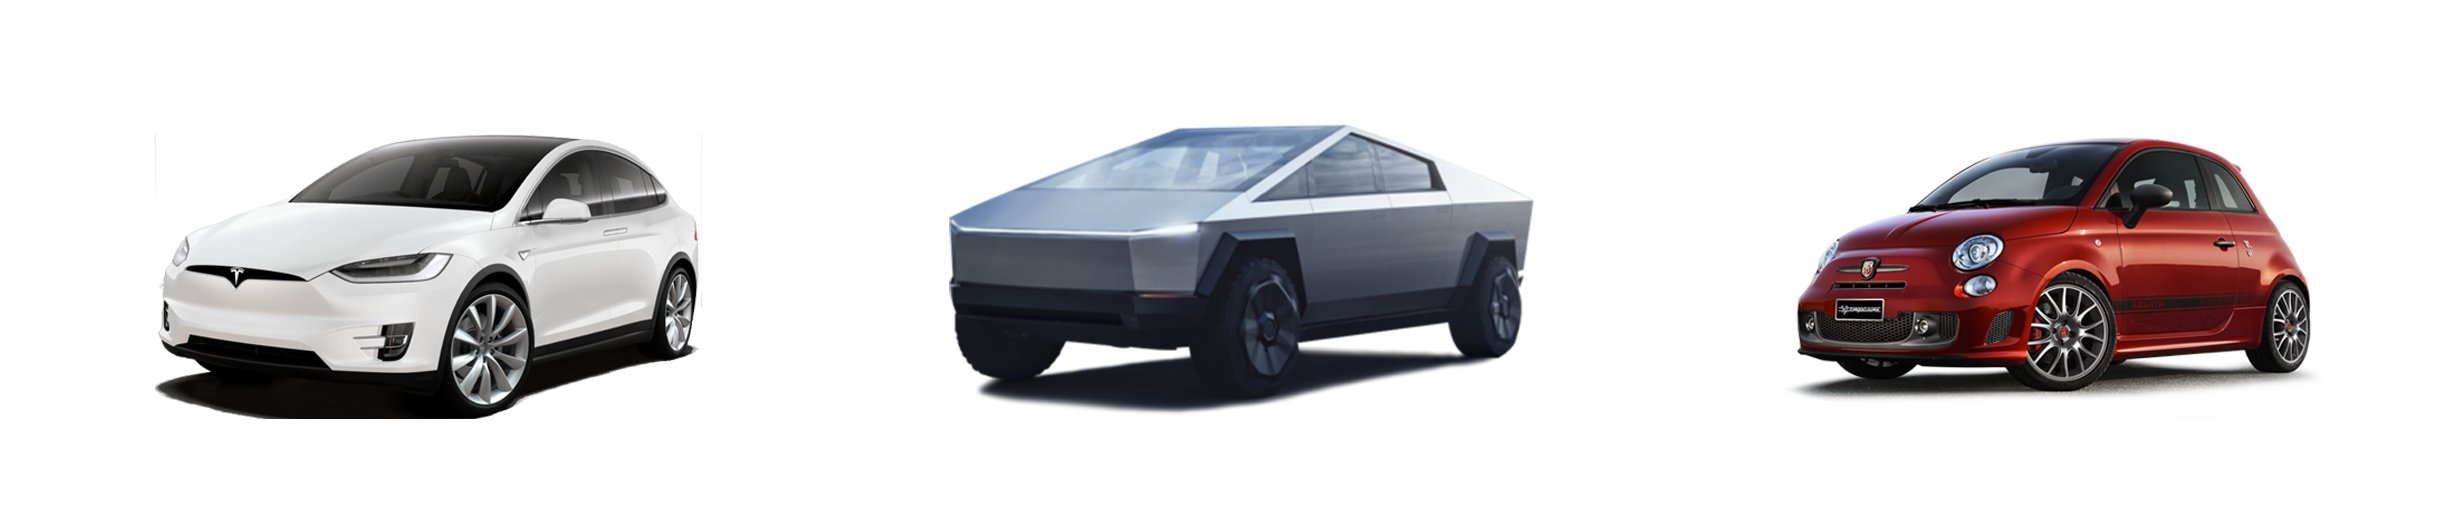
\includegraphics[width = 0.9\linewidth]{AUTO.png}
            \centering
            \caption{Esempio di veicoli con feature differenti ma appartenenti alla stessa categoria (automobile)}
            \label{auto}
        \end{figure}
        \item \emph{Condizioni dell’immagine}: Oltre al concetto temporale, i motivi che 
        portano ad una variabilità intra-calasse possono essere l’occlusione, 
        l’illuminazione, posa, punto di vista, ambiente circostante, condizioni 
        meteorologiche etc. Questi fattori influenzanti possono incidere 
        negativamente sull’aspetto di un oggetto. Ulteriori problematiche possono 
        riguardare l’aggiunta di artefatti di digitalizzazione, presenza del 
        rumore, bassa risoluzione e distorsioni varie (Fig. \ref{agenti atmosferici}).
        \begin{figure}[H]
            \centering
            \hspace*{1.7cm}
            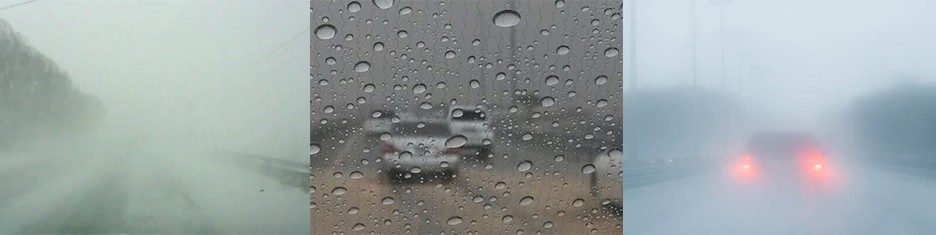
\includegraphics[width = 0.8\linewidth]{nebbia.png}
            \centering
            \caption{Esempio di immagini con scarsa visibilità e a basso contenuto informativo.}
            \label{agenti atmosferici}
        \end{figure}
    \end{enumerate}
    \item \emph{Numero di categorie}: il numero di classi può rilevarsi un problema quando 
    queste sono numerose. Un elevato numero di classi, oltre che ad aumentare 
    la probabilità di avere una bassa variabilità inter-calasse, richiede un alto 
    numero di etichette che a loro volta sono difficili da reperire. In questo caso 
    è favorita un’alta variabilità inter-classe (oggetti diversi appartenenti a classi 
    diverse). Ad oggi, l’utilizzo dell’esatto numero di esempi per addestrare un 
    modello è una domanda di ricerca ancora aperta;
    \item \emph{Efficienza}: attualmente non è possibile eseguire un modello complesso su 
    dispostivi sprovvisti di elevate risorse di calcolo. La ricerca è rivolta nell’ottimizzazione 
    di tali modelli affinché questi vengano eseguito anche su dispositivi mobili.
\end{itemize}
Le prestazioni di un modello vengono calcolate utilizzando alcune metriche, come 
per esempio i \emph{Frame Per Secondo (FPS)}, \emph{Precisione} e \emph{Recall}, ma la più usata è la 
\emph{mean Average Precision (mAP)}. La precisione misura la percentuale di previsioni 
corrette mentre il richiamo misura le previsioni corrette rispetto alla verità 
di base (\emph{ground truth}).
\begin{eqnarray}\label{precision}
    Precision & = & \frac{True \ Positive}{True \ Positive + False \ Positive} \nonumber \\
             & = & \frac{True \ Positive}{All \ Observations}
\end{eqnarray}
\begin{eqnarray}\label{recall}
    Recall & = & \frac{True \ Positive}{True \ Positive + False \ Negative} \nonumber \\
             & = & \frac{True \ Positive}{All \ Ground \ Truth}
\end{eqnarray}
Gli output standard di un rilevatore, su un’immagine di test $I$, al fine di 
identificare un oggetto $j$, sono:
\begin{itemize}
    \item $b_j$: \emph{Bounding-Box (BB)} disegnata sull’oggetto di interesse;
    \item $c_j$: categoria predetta;
    \item $p_j$: livello di confidenza che verrò comparato con una soglia $\beta$ per determinare 
    l’accettabilità o meno dell’etichetta della classe predetta. 
\end{itemize}
Una predizione $(b,c,p)$ è considerata come un vero positivo $(TP)$ se:
\begin{enumerate}
    \item La categoria predetta $c$ è uguale all’etichetta $c_g$ fornita nel ground truth;
    \item \emph{L'Intersection Over Union (IoU)} (\ref{iou}), è maggiore di una soglia $\epsilon$. L'IoU 
    rappresenta il rapporto tra l'area della bounding box predetta $b$ e l'area 
    della bounding box $b_g$ presente nel ground truth, dove $\cap$ e $\cup$ indicano 
    rispettivamente l’intersezione e l’unione delle varie aree.
    \begin{eqnarray}\label{iou}
        IoU(b,b_g) & = & \frac{area(b \cap b_g)}{area(b \cup b_g)} \nonumber \\
                 & = & \frac{Area \ of \ overlap}{Area \ of \ union}
    \end{eqnarray}
    Quando il modello prevederà una bounding box con un valore IoU maggiore 
    o uguale alla soglia,  tipicamente pari a 0.5, allora questo vuol dire che ci 
    sarà un’elevata sovrapposizione tra questa e una delle bounding box presenti 
    nel ground truth. D’altra parte, quando il valore di IoU è minore della 
    soglia, questo sintomo sarà ritenuto come una previsione errata da parte 
    del modello in quanto non c’è sovrapposizione fra le varie bounding box. 
    Questo comportamento fa si che la regione rilevata venga classificata come 
    un Falso Positivo \emph{(FP)}. Se invece il modello non riesce a rilevare un oggetto 
    presente nell’immagine, allora si parlerà di Falso Negativo $(FN)$.
    \begin{equation}\label{iou values}
        class(IoU) = \left\{
            \begin{array}{rl}
            TP & \mbox{if } IoU \geq \epsilon \\
            FP & \mbox{if } IoU < \epsilon \\
            FN & \mbox{if } IoU = \emptyset
            \end{array}
            \right.
    \end{equation}
\end{enumerate}
A questo punto, per poter calcolare l’Average Precision, consideriamo la $IoU$ come 
la nostra precisione \cite{rosebrock2017deep}. L’average precision, calcolata su una singola classe $i$, sarà 
quindi definita come:
\begin{equation}\label{average precision}
    AP_i = \frac{IoU}{L_i}
\end{equation}
Dove $L_i$ rappresenta il numero totale delle label appartenenti a una specifica classe 
$i$. La \emph{mean Average Precision (mAP)} sarà possibile calcolarla con la seguente formula:
\begin{equation}\label{mean average precision}
    mAP = \frac{1}{N}\sum_{i=1}^NAP_i
\end{equation}
dove N rappresenta il numero totali di classi.

\subsection{Image Segmentation}
Nella Figura (\ref{segmentation}) è stato introdotto brevemente l’argomento della segmentazione 
delle immagini.  I recenti risultati, raggiunti nella segmentazione delle immagini, 
derivano dai progressi svolti nell’ottimizzazione delle \emph{Deep Convolutional Neural 
Networks (DCNN)}, in particolare dalle Convolutional Neural Networks (CNN). 
Nel 1989, sempre LeCun inventò \emph{LeNet-5} \cite{LeNet-5}, una rete neurale convoluzionale 
sviluppata per riconoscere i numeri scritti a mano. Grazie a questa, venne spianata 
la strada verso il continuo successo delle CNN nello svolgere vari compiti di visione 
artificiale di alto livello, oltre che a motivare i ricercatori ad esplorare le capacità 
di tali reti per problemi di classificazione pixel-wise, come la segmentazione delle 
immagini. La segmentazione di un’immagine è uno dei  compiti indispensabili 
nella visione artificiale in quanto è utile in diversi campi scientifici, come per 
esempio la guida autonoma, ambito medico, ambito biometrico, ambito militare, 
riconoscimento etc. Per poter svolgere questo complicato compito, a differenza 
della classificazione e dell’object detection, è necessario reperire delle informazioni 
spaziali di basso livello o a livello di pixel.
L’image segmentation si suddivide in due categorie:
\begin{enumerate}
    \item \emph{Semantic segmentation}
    \item \emph{Instance segmentation}
\end{enumerate}
Esiste un’ulteriore categoria, chiamata \emph{Panoptic Segmentation}, derivata dalla 
fusione dei risultati provenienti dalle due principali categorie. In questo elaborato 
verrà discussa solamente la tecnica di Semantic Segmentation. prima di introdurre 
la tecniche citata, è doveroso specificare che la segmentazione delle immagini è 
un argomento trattato anche nell’elaborazione dei video.

\subsubsection{Semantic Segmentation}
Il deep learning ha fortemente promosso la ricerca sulla segmentazione semantica. 
La comunità industriale sta facendo enormi sforzi nello sviluppo di sistemi avanzati 
in grado di effettuare una segmentazione semantica. Per esempio, una fotocamera, 
installata nei diffusi dispositivi mobili, è in grado di produrre un ritratto mediante 
l’effetto di profondità, comunemente chiamato effetto bokeh, incorporando la tecnica 
di segmentazione. Nella segmentazione semantica ogni pixel viene classificato 
in base alla classe di appartenenza dell’oggetto presente nell’immagine (es: strada, 
automobile, pedone, edificio etc.). In questo caso, i pixel dell’immagine aventi la 
stessa etichetta, condividono determinate caratteristiche come colore, intensità, 
consistenza etc. In altre parole, la segmentazione semantica tende a suddividere 
l’immagine in sottoinsiemi che si escludono a vicenda, in cui ogni sottoinsieme 
rappresenta una regione significativa dell’immagine originale. Rispetto alle altre 
tecniche, la tecnica di semantic segmentation ha esigenze più elevate in quanto 
non si limita solamente a classificare gli oggetti presenti (image classification) e a 
rilevarne la loro posizione (object detection) mediante delle bounding box, ma 
mira a partizionare ogni regione dell’oggetto (foreground) rispetto alla regione 
di sfondo (background). Per esempio, le auto presenti nella Figura (\ref{semantic segmentation}), vengono 
raggruppate come un unica porzione di pixel \cite{aurelien}.
\begin{figure}[H]
    \centering
    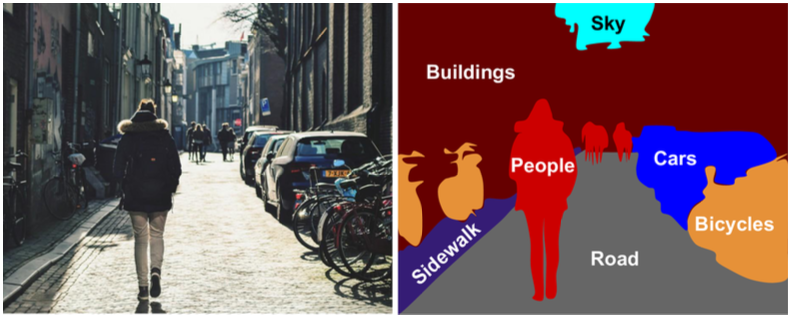
\includegraphics[width = 0.9\linewidth]{sem seg.png}
    \centering
    \caption{Esempio Semantic segmentation.}
    \label{semantic segmentation}
\end{figure}
Allo stato dell’arte esistono varie tipologie di architetture di reti neurali 
comunemente utilizzate per produrre delle segmentazioni semantiche \cite{semantic_segmentation_networks}:
\begin{enumerate}
    \item \emph{Fully convolutional networks (FCN)}
    \item \emph{Dilation/Atrous convolution}
    \item \emph{Top-Down/Bottom-up approach}
    \item \emph{Global Context}
    \item \emph{Receptive field enlargement and multi-scale context incorporation}
\end{enumerate}

\subsubsection{FULLY CONVOLUTIONAL NETWORKS}
Long et al. \cite{fcn} propose la pietra miliare Fully Convolutional Network (FCN), 
che diede un gran contributo all’incremento dell’accuratezza della segmentazione 
semantica. Lo studio si basò sull’utilizzo di svariati classificatori come: AlexNet \cite{alexnet}, 
VGGNet\cite{vggNet} e GoolgeNet \cite{googleNet}, tutte pre-addestrare con gli stessi dati. 
Ogni classificatore, come precedentemente spiegato in \ref{RNC}, ha lo scopo di prendere 
un'immagine in input e ridimensionarla tramite l’attraversamento dei layer 
convoluzionali, fino a giungere ai layer fully connected (FC). L’output prodotto 
sarà sotto forma di label predetta (Fig. \ref{CNN complete}). Per convertire questi modelli da 
classificatori a modelli FCN densi, bisogna sostituire i layer fully connected con 
layer convoluzionali di dimensione $1 \times 1 \times 21$, dove 21 rappresenta il numero delle 
classi esistenti in PASCAL VOC (20), più la classe di background. Tramite una 
procedura di \emph{Upsampling}, viene effettuata un’operazione di \emph{deconvoluzione}, spesso 
chiamata \emph{convoluzione trasposta}, utile a restituire in ouput l’immagine di partenza 
ricostruita. Esistono varie tipologie di upsampling, fra queste abbiamo:
\begin{enumerate}
    \item \emph{Nearest-Neighboor}: Copia il valore del pixel più vicino;
    \item \emph{Up-Sampling Bilineare}: calcola il valore dei pixel attraverso l’interpolazione lineare e l’uso dei pixel adiacenti;
    \item \emph{Up-sampling Bicubico}: Calcola il valore dei pixel attraverso l’interpolazione polinomiale. Questa operazione ha un alto tasso computazionale ma allo stesso tempo produce risultati migliori rispetto alle sue concorrenti. 
\end{enumerate}
Quando si sarà giunti a un layer di pooling pari alla dimensione di $1 \times 1$, allora 
si potrà attuare l’upsampling per poter ricostruire l’immagine di partenza (Fig. \ref{FCN}). 
\begin{figure}[H]
    \centering
    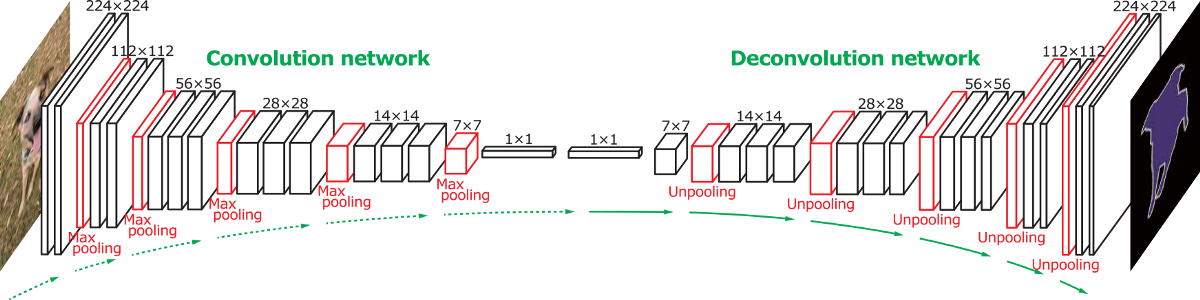
\includegraphics[width = \linewidth]{FCN.png}
    \centering
    \caption{Esempio di architettura Fully Convolutional Network}
    \label{FCN}
\end{figure}
Tale architettura è composta da un \emph{Encoder} e da un \emph{Decoder}.
\begin{itemize}
    \item \emph{Encoder}: sezione dell’architettura adibita all’estrazione del contesto dell’immagine. 
    La sua struttura è composta da livelli di convoluzione e di max 
    pooling, come una comune CNN, che riducono (down-sample) l’immagine 
    in ingresso; 
    \item \emph{Decoder}: sezione dell’architettura adibita alla localizzazione degli elementi 
    presenti nell’immagine attraverso l’utilizzo di convoluzioni trasposte. Il compito 
    di un decoder è quello di amplificare le feature map tramite operazioni 
    di deconvoluzione utili a ricostruire l’immagine di ingresso includendone i 
    suoi artefatti.
\end{itemize}
Esitono diverse reti FCN che adottano questa tipologia di architettura. Per 
quanto riguarda le operazioni svolte, un confronto tra l’operazione di Pooling 
(downsampling) e di Unpooling (upsampling), o di convoluzione e deconvoluzione, 
sono mostrate nella Figura \ref{deconvolution}.
\begin{figure}[H]
    \centering
    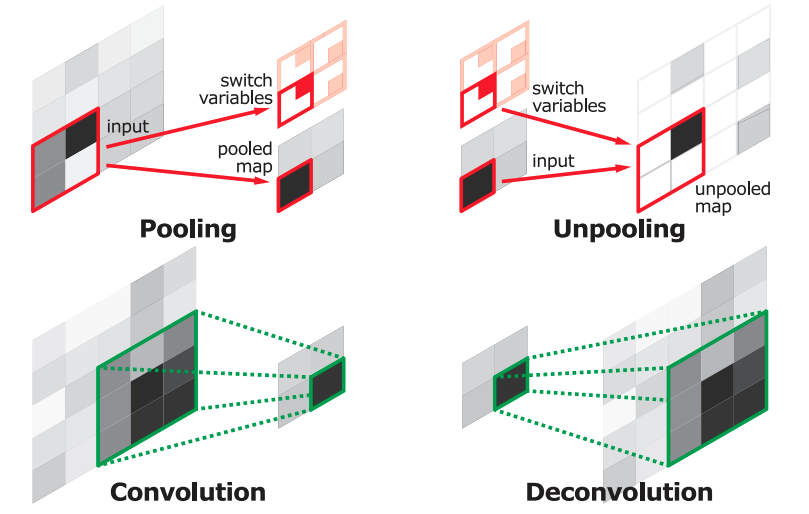
\includegraphics[width = 0.7\linewidth]{deconvolution.png}
    \centering
    \caption{Esempio di Deconvoluzione e di Unpooling (Upsampling).}
    \label{deconvolution}
\end{figure}
In base al numero di layer convoluzionali presenti, esistono diverse architetture 
di Fully Convolutional Networks. Una fra queste, la \emph{FCN-32}, è composta da 
un encoder che ha il compito di ridurre l’immagine iniziale di 32 volte e da un 
decoder che svolgerà il processo inverso di ricostruzione. Avendo pochi dati a 
disposizione, la rete farà fatica a ricostruire un output simile a all’input, questo si 
verifica a causa della perdita delle informazione significative nel processo svolto 
dall’encoder. Per avere una rappresentazione più fedele dell’immagine in output, 
ci corrono in auto altre due tipologie di architetture: \emph{FCN-16} e \emph{FCN-8}.
\begin{figure}[H]
    \centering
    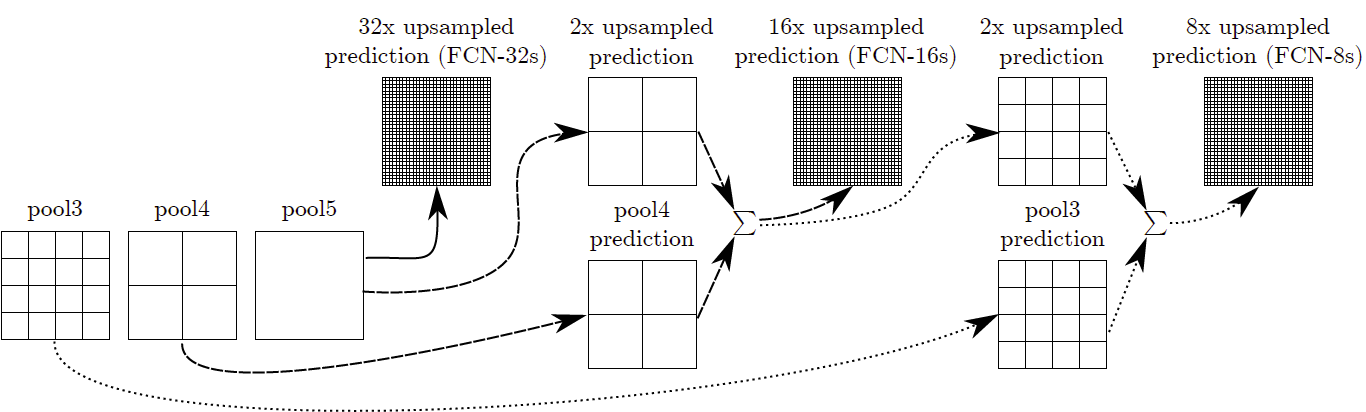
\includegraphics[width = \linewidth]{FCN-32.png}
    \centering
    \caption{Esempio derivazione delle varie architetture FCN.}
    \label{FCN-models}
\end{figure}
Quest’ultime utilizzano una strategia intelligente per poter ricostruire l’immagine. 
Per giungere a un buon risultato, oltre che a fare riferimento alla sola feature 
map, utilizzano i livelli di pooling precedenti nella quale ci sono maggiori informazioni. 
Per giungere ad un’architettura FCN-8, bisognerà svolgere un processo 
iterativo che va ad effettuare una somma di ogni singolo elemento (element-wise) 
tra l’upsampling del pooling layer $n$ con il pooling layer $n-1$. La ricostruzione 
risultante sarà quella più fedele al ground truth. Questa architettura 
ha permesso di convertire i modelli precedenti in \emph{FCN-AlexNet}, \emph{FCN-VGG16} e 
\emph{FCN-GoogleNet}.

\subsubsection{DILATATION/ATRUS CONVOLUTION}
\subsubsection{DilatedNet}
Per rimediare alla bassa qualità prodotta in output da una comune rete CNN, Yu 
e Koltun introdussero un versione modificata chiamata {\bfseries{Convoluzione Dilatata}} 
o {\bfseries{DilatedNet}} \cite{DilatedNet}. Questo modello consentiva di estrarre le informazioni che 
consentivano una migliore segmentazione che non comportasse a sua volta alla 
perdita di dati rilevanti. L’idea della Convoluzione dilatata, chiamata anche 
\emph{Convoluzione Atroce}, deriva dalla decomposizione wavelet. A differenza del 
tradizionale operatore di convoluzione, la convoluzione dilatata introduce un tasso 
di dilatazione \emph{(dilated rate)} $l$, utile a saltare alcuni punti, presenti nel 
campo ricettivo, durante la convoluzione. La formula matematica per il calcolo della 
convoluzione dilatata è la seguente:
\begin{equation}
    (F*_lk)(p) = \sum_{s+lt=p}F(s)k(t)
\end{equation}
dove:
\begin{equation}\label{dilated rate}
    Conv(l) = \left\{
        \begin{array}{rl}
        Standard & \mbox{if } l = 1\\
        Dilated & \mbox{if } l > 1
        \end{array}
        \right.
\end{equation}
Con un dilated rate pari a 2, otterremmo la seguente convoluzione dilatata (Fig. (\ref{dilated})):
\begin{figure}[H]
    \centering
    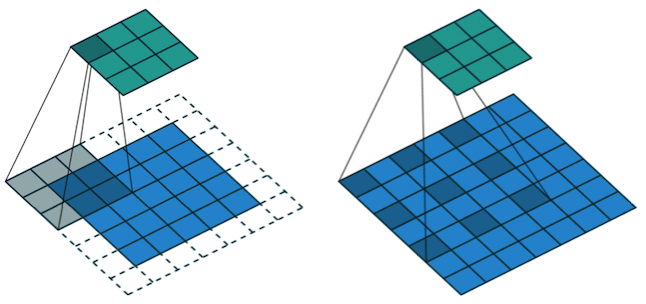
\includegraphics[width = 0.8\linewidth]{dilated.png}
    \centering
    \caption{Esempio di convoluzione standard ($l=1$)(Sinistra) e di Convoluzione Dilatata ($l=2$) (Destra).}
    \label{dilated}
\end{figure}
Maggiore sarà il valore del tasso di dilatazione, maggiore sarà il campo ricettivo 
e minore saranno i calcoli da svolgere. 

\subsubsection{DeepLab}
DeepLab è un modello utilizzato allo stato dell’arte per la segmentazione semantica 
progettato da Google. Per la costruzione della rete sono state affrontate due 
problematiche: il down-sampling e l’invarianza spaziale. Il primo problema, legato 
alla riduzione della risoluzione delle feature, è stato risolto grazie all’applicazione 
dell’algoritmo soprannominato “atroce”. Ogni encoder è composto dalla combinazione 
di layer di pooling che riducono la risoluzione spaziale delle feature map. 
Per poter ricostruire le informazioni perse, si può utilizzare la deconvoluzione. 
Quest’ultima richiede però un quantitativo importante di memoria e di tempo. 
L’algoritmo atroce offre un metodo alternativo alla deconvoluzione. Il suo scopo 
è quello di applicare una convoluzione che permetta di allargare efficacemente il 
campo visivo dei filtri senza aumentare il numero di parametri preservando la 
quantità di computazione richiesta. La tecnica della convoluzione atrosa può essere 
vista come come un espediente della tecnica di upsampling. Per poter risolvere il 
secondo problema, legato alla precisione ridotta a causa dell’invarianza spaziale, 
questa tipologia di rete, al fine di catturare dettagli più fini, applica un \emph{Conditional 
Random Field (CRF)} completamente connesso. Questa classe di modelli 
discriminanti utilizzano le informazioni contestuali delle label per effettuare delle 
buone previsioni. Restando ad un discorso più ad alto livello, le potenzialità del 
CRF riguardano l’utilizzo di termini leviganti (\emph{smoothness}) utili a massimizzare la 
relazione tra le etichette di pixel simili che esaltano il foreground dal background. 
Questi termini permetto quindi di avere una mappa di segmentazione migliore 
anche dopo aver applicato poche volte, in maniera iterativa, l’algoritmo del CRF. 
L’architettura generale di un modello DeepLab consiste nel prendere in input 
un’immagine e di elaborarla da una comune DCNN in cui ci sono degli strati 
atrosi, per poter generare una prima Score map su cui verrà fatto l’upsampling 
con un’interpolazione bilineare. Dopo aver estratto un’immagine avente le stesse
dimensioni dell’immagine di partenza, verrà applicato il CRF.
\begin{figure}[H]
    \centering
    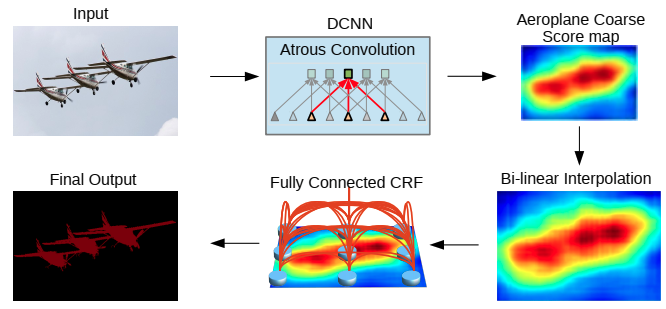
\includegraphics[width = \linewidth]{CRF.png}
    \centering
    \caption{Esempio architettura DeepLab.}
    \label{CRF}
\end{figure}

\subsubsection{TOP-DOWN/BOTTOM-UP APPROACH}
\subsubsection{U-Net}
La rete U-Net \cite{unet} è una rete di segmentazione semantica, con una architettura a forma 
di U (Fig. (\ref{unet})) composta anch’essa da un encoder, o percorso di contrazione, e 
un decoder, o percorso di espansione.
\begin{figure}[H]
    \centering
    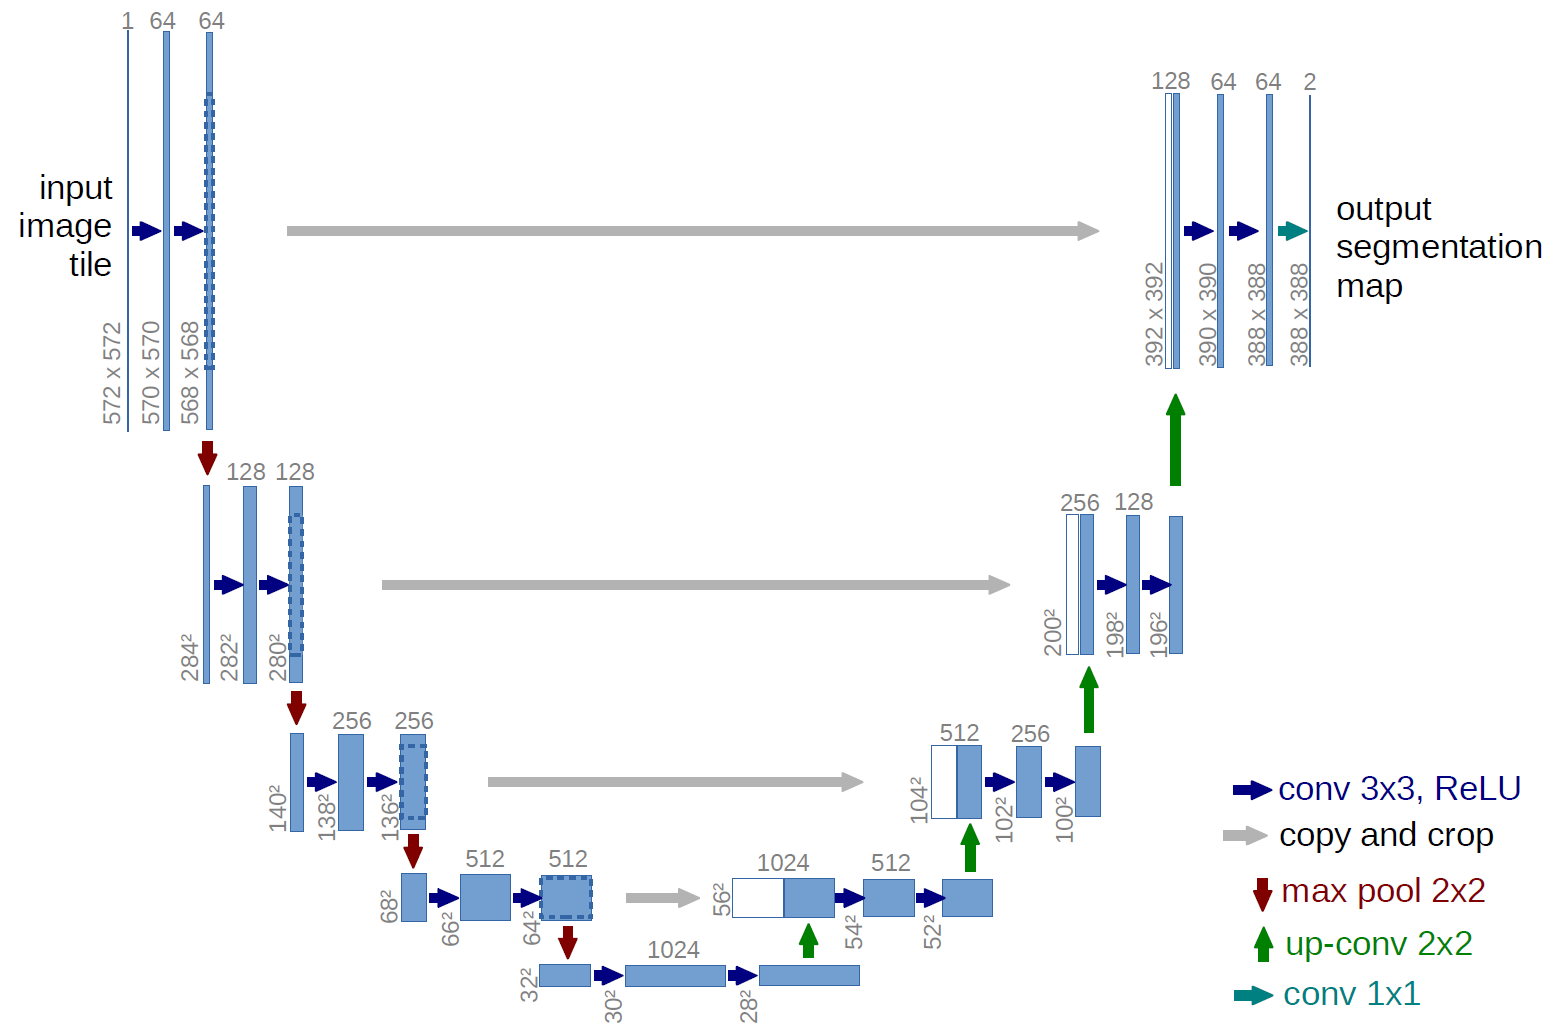
\includegraphics[width = \linewidth]{Unet.png}
    \centering
    \caption{Esempio architettura rete U-Net.}
    \label{unet}
\end{figure}
Nell’immagine, ogni riquadro blu rappresenta una feature map multicanale. Il 
numero dei canali (specificati sopra ogni riquadro) e le dimensioni (specificate in 
basso a sinistra di ogni riquadro), variano in base alla profondità della rete. I 
riquadri bianchi, presenti nello strato di decoder, stanno a rappresentare le feature 
map copiate dallo strato dell’encoder. Fra i vari layer esistenti in entrambe le 
parti, esistono delle connessioni, chiamate \emph{Shortcut connection}, capaci di creare 
un collegamento utile a trasferire le informazioni estratte dall’encoder verso il 
decoder. Questi collegamenti sono utili a velocizzare il processo di up-sampling e 
migliorare nel contempo il risultato finale. La sezione dell’encoder è formata da 
due convoluzioni $3 \times 3$ consecutive, seguite dalla funzione di attivazione ReLU e 
da un’operazione di max-pooling avente una finestra di dimensioni $2 \times 2$ con 
passo 2. Dalla parte del decoder invece abbiamo l’operazione di up-sampling delle 
feature map seguita da una deconvoluzione $2 \times 2$. La mappa delle caratteristiche 
risultati viene concatenata con la mappa delle caratteristiche ritagliata estratta 
dall’encoder. Successivamente, vengono applicate due operazione di convoluzioni 
consecutive aventi finestra di dimensione pari a $3 \times 3$.

\subsubsection{SegNet}
Così come i modelli già visti, anche SegNet ha un’architettura composta da un 
encoder e un decoder. La parte adibita all’encoder utilizza 13 layer convoluzionali, 
mentre la parte destinata al decoder contiene anch’essa 13 layer per la deconvoluzione. 
In ogni layer della sezione encoder, viene utilizzato un banco di filtri 
per produrre le feature map. Per poter ridurre lo spostamento della covarianza 
interna, problema legato all’input che porta la rete a non essere abbastanza 
efficiente e/o ad avere una scarsa generalizzazione, viene utilizzata una tecnica 
nota come batch normalization \cite{batchNorm} seguita da una funzione attivazione ReLU. Su 
ogni feature map viene applicato un max-pooling con una finestra di dimensioni 
$2\times 2$ e passo 2. Come già noto, un alto numero di operazioni si sub-sampling 
comporta una maggiore precisione di classificazione, ma allo stesso tempo provoca 
una riduzione di ogni feature map che, tradotto in altri termini, causa la perdita 
dei dati. La riduzione del numero di dati determina la creazione di bordi sfocati 
il quale rappresenta un problematica centrale per un’operazione di segmentazione. 
Per risolvere il problema della perdita dei dati, SegNet effettua solo una memorizzazione 
degli indici di pooling per ciascuna feature map prodotta dall’encoder. 
Tali indici saranno utili al decoder per effettuare l’operazione di upsampling 
al fine di costruire delle feature map ad alta risoluzione che avessero l’obiettivo di 
produrre un’immagine in output avente le stesse dimensioni di quella in input. 
Per giungere al risultato finale, anche il decoder utilizza un banco di filtri, a loro 
volta aggiornabili in fase di addestramento, per poter effettuare la deconvoluzione. 
La feature map prodotta da un decoder verrà inserità in un classificatore softmax 
multi-classe addestrabile che effettuerà l’etichettatura di ogni singolo pixel.
\begin{figure}[H]
    \centering
    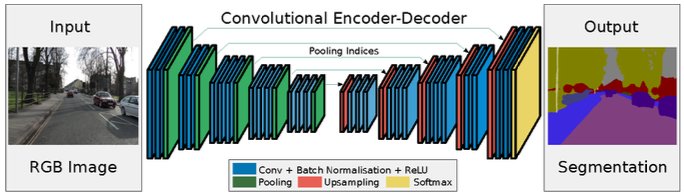
\includegraphics[width = \linewidth]{segnet.png}
    \centering
    \caption{Esempio architettura rete SegNet.}
    \label{segnet}
\end{figure}

\subsubsection{GLOBAL CONTEXT}
\subsubsection{ParseNet}
Un significativo miglioramento delle reti FCN ebbe inizio con l’introduzione della 
rete ParseNet \cite{parsenet}. Codesta, a differenza delle reti FCN, utilizza le informazioni 
inerenti le feauture globali, o contesto globale, per poter produrre in output una 
buona segmentazione dell’immagine (Fig. (\ref{global context})).
\begin{figure}[H]
    \centering
    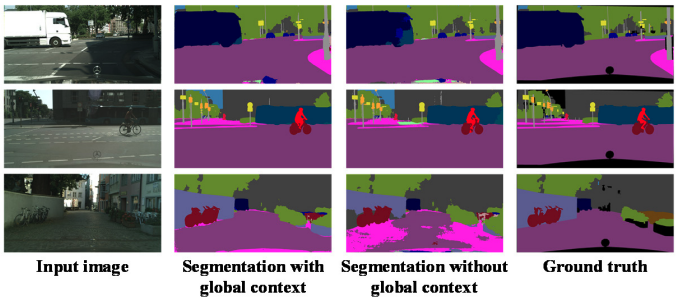
\includegraphics[width = \linewidth]{gloabal context.png}
    \centering
    \caption{Esempio di applicazione del contesto globale alla segmentazione.}
    \label{global context}
\end{figure}
Le feature globali sono utili per poter rappresentare un oggetto nella sua 
totalità. Per poter ricavare queste informazioni, vengono utilizzate delle feature 
map sulla quale viene eseguito il pooling mediante una media globale. Dopo aver 
effettuato il pooling, viene eseguita l’operazione inversa (\emph{un-pooling}) per poter 
riportare l’immagine alle sue dimensioni di partenza. Successivamente, le feature 
map di partenza e quelle ricavate vengono combinate per effettuare una previsione 
sul punteggio di classificazione finale. Ogni feature map appartiene a un layer 
diverso, pertanto la combinazione di queste sarà formata da feature map diverse 
in termini di scala e di norma. Affinché tutto funzioni, vengono applicate due 
normalizzazioni L2 (\ref{L2}), una dopo il pooling globale e l’altra dopo la feature 
map di partenza estratta contemporaneamente dalla FCN. 
\begin{equation}\label{L2}
    \norm{x}_2 = \left(\sum_{i=1}^d \abs{x_i}^2 \right)^\frac{1}{2}
\end{equation}
Dove $x$ rappresenta l’input e $d$ rappresenta la sua dimensionalità. Nel percorso 
inferiore, viene eseguita una normalizzazione L2, a ciasun livello di convoluzione, 
per ciascun canale. Nel percorso superiore invece, viene effettuato un pooling 
medio delle feature map in ogni specifico livello di convoluzione. Dopo aver 
ottenuto le feature globali, viene effettuata una normalizzazione L2. L’unpooling 
è utile a poter far combaciare le dimensioni dei vettori superiori con i vettori 
inferiori, in modo che questi possano essere concatenati. La figura (\ref{parsenet}) riassume 
i passaggi precedenti.
\begin{figure}[H]
    \centering
    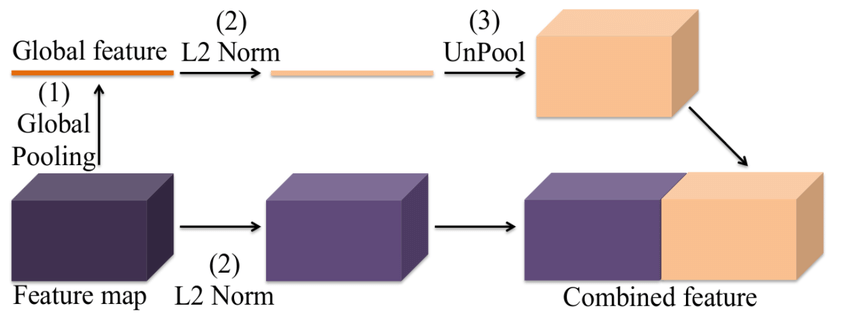
\includegraphics[width = 0.8\linewidth]{parsenet.png}
    \centering
    \caption{Modulo ParseNet.}
    \label{parsenet}
\end{figure}

\subsubsection{GCN}
La segmentazione semantica basa il suo principio di funzionamento su due aspetti: 
classificazione e localizzazione. Quest’ultimi sono ritenuti come due concetti 
di natura opposta in quanto, una piccola trasformazione dell’input, come ad 
esempio una traslazioni o rotazioni, rende la classificazione invariante mentre, allo 
stesso tempo, la localizzazione potrebbe risentirne negativamente, pertanto risulta 
essere più sensitiva rispetto alla classificazione. Per sopperire alle problematiche 
delle trasformazioni su entrambe le tecniche, venne introdotto il modello \emph{Global 
Convolutional Network (GCN)} \cite{gcn}. La rete è basata sui seguenti due principi:
\begin{enumerate}
    \item Dal punto di vista della \emph{localizzazione}, la struttura del modello dev’essere 
    completamente convolutiva per poter mantenere le informazioni utili alla 
    localizzazione degli oggetti in quanto, se la struttura fosse stata a livelli 
    completamente connessi (fully-connected layers), o pooling globali, questi 
    scarterebbero tutte le informazioni spaziali;
    \item Dal punto di vista della \emph{classificazione}, devono essere utilizzati dei kernel 
    di grandi dimensioni, circa $15\times 15$, al fine di consentire la realizzazione di 
    connessioni dense tra le feature map e le classificazioni pixel-wise. Questi 
    filtri consentono di effettuare delle convoluzioni globali che rendono la rete 
    invariante alle trasformazioni.
\end{enumerate}
Per poter migliorare il contorno della segmentazione, viene utilizzata il blocco 
\emph{Boundary Refinement (BR)} dopo l’applicazione del modulo GCN e durante 
il processo di deconvoluzione.
\begin{figure}[H]
    \centering
    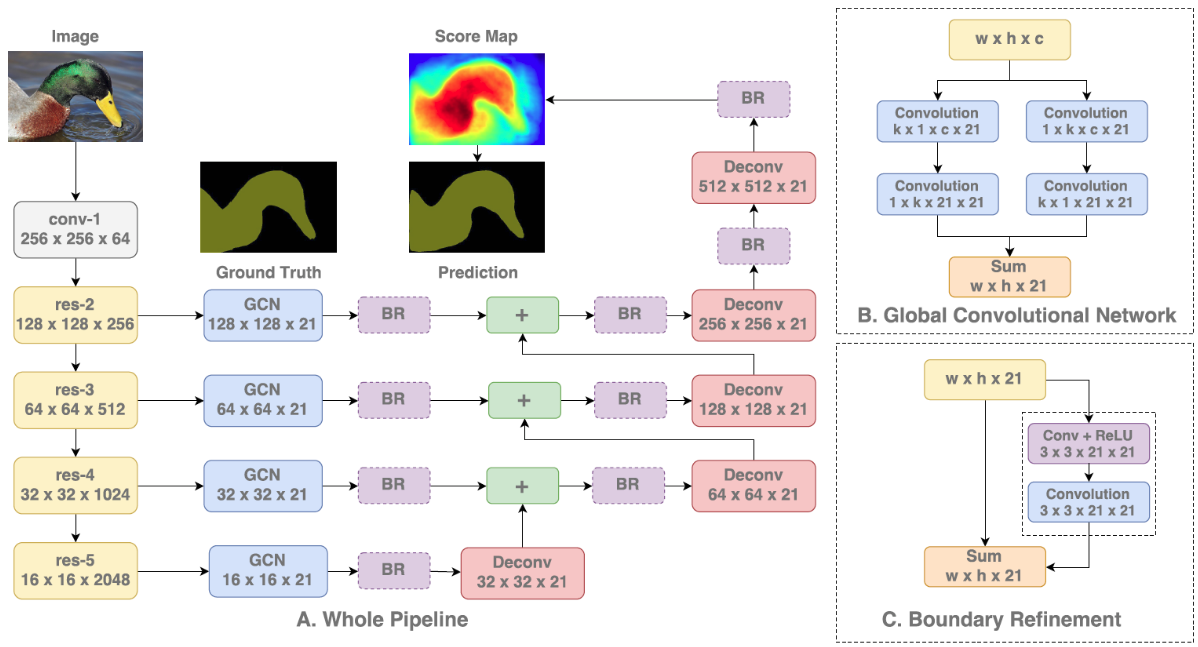
\includegraphics[width = \linewidth]{GCN.png}
    \centering
    \caption{Architettura modello GCN.}
    \label{gcn}
\end{figure}
Come visto in Figura (\ref{gcn}), ResNet è la rete che viuene utilizzata come 
backbone (spina dorsale), pre-addestrata con le immagini contenute nel dataset 
ImageNet. Sulle mappe dei punteggi di bassa risoluzione viene effettuata un’operazione di upsampling con un layer di deconvoluzione. Le mappe ottenute dalla deconvoluzione verranno aggiunte con quelle più alte per poter generare nuove mappe dei punteggi utili alla segmentazione finale.
